\documentclass[]{article}
\usepackage{lmodern}
\usepackage{amssymb,amsmath}
\usepackage{ifxetex,ifluatex}
\usepackage{fixltx2e} % provides \textsubscript
\ifnum 0\ifxetex 1\fi\ifluatex 1\fi=0 % if pdftex
  \usepackage[T1]{fontenc}
  \usepackage[utf8]{inputenc}
\else % if luatex or xelatex
  \ifxetex
    \usepackage{mathspec}
  \else
    \usepackage{fontspec}
  \fi
  \defaultfontfeatures{Ligatures=TeX,Scale=MatchLowercase}
\fi
% use upquote if available, for straight quotes in verbatim environments
\IfFileExists{upquote.sty}{\usepackage{upquote}}{}
% use microtype if available
\IfFileExists{microtype.sty}{%
\usepackage{microtype}
\UseMicrotypeSet[protrusion]{basicmath} % disable protrusion for tt fonts
}{}
\usepackage[margin=1in]{geometry}
\usepackage{hyperref}
\hypersetup{unicode=true,
            pdfborder={0 0 0},
            breaklinks=true}
\urlstyle{same}  % don't use monospace font for urls
\usepackage{color}
\usepackage{fancyvrb}
\newcommand{\VerbBar}{|}
\newcommand{\VERB}{\Verb[commandchars=\\\{\}]}
\DefineVerbatimEnvironment{Highlighting}{Verbatim}{commandchars=\\\{\}}
% Add ',fontsize=\small' for more characters per line
\usepackage{framed}
\definecolor{shadecolor}{RGB}{248,248,248}
\newenvironment{Shaded}{\begin{snugshade}}{\end{snugshade}}
\newcommand{\KeywordTok}[1]{\textcolor[rgb]{0.13,0.29,0.53}{\textbf{#1}}}
\newcommand{\DataTypeTok}[1]{\textcolor[rgb]{0.13,0.29,0.53}{#1}}
\newcommand{\DecValTok}[1]{\textcolor[rgb]{0.00,0.00,0.81}{#1}}
\newcommand{\BaseNTok}[1]{\textcolor[rgb]{0.00,0.00,0.81}{#1}}
\newcommand{\FloatTok}[1]{\textcolor[rgb]{0.00,0.00,0.81}{#1}}
\newcommand{\ConstantTok}[1]{\textcolor[rgb]{0.00,0.00,0.00}{#1}}
\newcommand{\CharTok}[1]{\textcolor[rgb]{0.31,0.60,0.02}{#1}}
\newcommand{\SpecialCharTok}[1]{\textcolor[rgb]{0.00,0.00,0.00}{#1}}
\newcommand{\StringTok}[1]{\textcolor[rgb]{0.31,0.60,0.02}{#1}}
\newcommand{\VerbatimStringTok}[1]{\textcolor[rgb]{0.31,0.60,0.02}{#1}}
\newcommand{\SpecialStringTok}[1]{\textcolor[rgb]{0.31,0.60,0.02}{#1}}
\newcommand{\ImportTok}[1]{#1}
\newcommand{\CommentTok}[1]{\textcolor[rgb]{0.56,0.35,0.01}{\textit{#1}}}
\newcommand{\DocumentationTok}[1]{\textcolor[rgb]{0.56,0.35,0.01}{\textbf{\textit{#1}}}}
\newcommand{\AnnotationTok}[1]{\textcolor[rgb]{0.56,0.35,0.01}{\textbf{\textit{#1}}}}
\newcommand{\CommentVarTok}[1]{\textcolor[rgb]{0.56,0.35,0.01}{\textbf{\textit{#1}}}}
\newcommand{\OtherTok}[1]{\textcolor[rgb]{0.56,0.35,0.01}{#1}}
\newcommand{\FunctionTok}[1]{\textcolor[rgb]{0.00,0.00,0.00}{#1}}
\newcommand{\VariableTok}[1]{\textcolor[rgb]{0.00,0.00,0.00}{#1}}
\newcommand{\ControlFlowTok}[1]{\textcolor[rgb]{0.13,0.29,0.53}{\textbf{#1}}}
\newcommand{\OperatorTok}[1]{\textcolor[rgb]{0.81,0.36,0.00}{\textbf{#1}}}
\newcommand{\BuiltInTok}[1]{#1}
\newcommand{\ExtensionTok}[1]{#1}
\newcommand{\PreprocessorTok}[1]{\textcolor[rgb]{0.56,0.35,0.01}{\textit{#1}}}
\newcommand{\AttributeTok}[1]{\textcolor[rgb]{0.77,0.63,0.00}{#1}}
\newcommand{\RegionMarkerTok}[1]{#1}
\newcommand{\InformationTok}[1]{\textcolor[rgb]{0.56,0.35,0.01}{\textbf{\textit{#1}}}}
\newcommand{\WarningTok}[1]{\textcolor[rgb]{0.56,0.35,0.01}{\textbf{\textit{#1}}}}
\newcommand{\AlertTok}[1]{\textcolor[rgb]{0.94,0.16,0.16}{#1}}
\newcommand{\ErrorTok}[1]{\textcolor[rgb]{0.64,0.00,0.00}{\textbf{#1}}}
\newcommand{\NormalTok}[1]{#1}
\usepackage{graphicx,grffile}
\makeatletter
\def\maxwidth{\ifdim\Gin@nat@width>\linewidth\linewidth\else\Gin@nat@width\fi}
\def\maxheight{\ifdim\Gin@nat@height>\textheight\textheight\else\Gin@nat@height\fi}
\makeatother
% Scale images if necessary, so that they will not overflow the page
% margins by default, and it is still possible to overwrite the defaults
% using explicit options in \includegraphics[width, height, ...]{}
\setkeys{Gin}{width=\maxwidth,height=\maxheight,keepaspectratio}
\IfFileExists{parskip.sty}{%
\usepackage{parskip}
}{% else
\setlength{\parindent}{0pt}
\setlength{\parskip}{6pt plus 2pt minus 1pt}
}
\setlength{\emergencystretch}{3em}  % prevent overfull lines
\providecommand{\tightlist}{%
  \setlength{\itemsep}{0pt}\setlength{\parskip}{0pt}}
\setcounter{secnumdepth}{5}
% Redefines (sub)paragraphs to behave more like sections
\ifx\paragraph\undefined\else
\let\oldparagraph\paragraph
\renewcommand{\paragraph}[1]{\oldparagraph{#1}\mbox{}}
\fi
\ifx\subparagraph\undefined\else
\let\oldsubparagraph\subparagraph
\renewcommand{\subparagraph}[1]{\oldsubparagraph{#1}\mbox{}}
\fi

%%% Use protect on footnotes to avoid problems with footnotes in titles
\let\rmarkdownfootnote\footnote%
\def\footnote{\protect\rmarkdownfootnote}

%%% Change title format to be more compact
\usepackage{titling}

% Create subtitle command for use in maketitle
\newcommand{\subtitle}[1]{
  \posttitle{
    \begin{center}\large#1\end{center}
    }
}

\setlength{\droptitle}{-2em}

  \title{}
    \pretitle{\vspace{\droptitle}}
  \posttitle{}
    \author{}
    \preauthor{}\postauthor{}
    \date{}
    \predate{}\postdate{}
  

\begin{document}

\begin{titlepage}

\center
\textsc{\LARGE University of Waterloo}\\[5cm]
{ \huge \bfseries Final Project Report}\\[4cm]
     \textsc{\Large STAT 331 Fall 2018}\\[3cm]
     
\emph{Group 91:}\\[0.5cm]
Gengyao \textsc{Yuan}(20613017)\\[0.5cm]
Shunyu \textsc{Zhao}(20699637)


\end{titlepage}

\tableofcontents

\newpage

\section{Summary}

The goal of the STAT 331 final project is to explore the relation of
healthy male single-fetus birth weight and some explanatory variables.
This report will be divided into 4 main sections:\\
Summary, which will cover the main purpose of the report and give a
brief explanation of how the project will analyze the data. Two
candidate models will be produced in the model selection section by
using the pre-fitting data diagnostic and automated model selection.
Model diagnostics section will perform an in-depth comparison of the two
candidates models by comparing different types of residual plots,
leverage and influence measures and cross-validation(rPMSE). In the end,
there will be a discussion section basing on the result of the most
likely linear model we get from the previous sections to talk about
several topics such like: ???what is the most important factors
associated with/influencing birth weight' After using serial statistical
analysis way that we learned in STAT 331 course, we find the fianl model
is like lm(formula = wt \textasciitilde{} gestation + parity + meth +
mage + mht + mwt + fht + fwt + income + time + number + gestation:income
+ mwt:income + gestation:mage + gestation:fwt + gestation:mwt +
gestation:fht + gestation:mht + fht:income, data = births\_clean)

\section{Model Selection}

\subsection{Brief data overview}

By view the summary of the data, we notice that there are several
illegal data. The domain of ``marital''(the mother's marital status) is
1 to 5, but it is clearly showing that there exist 0 in ``marital,'' we
replace all the 0 to NA since it is not available data(out of range).\\
For the categorical predictor ``meth''(The self-reported ethnicity of
the mother) and ``feth''(The self-reported ethnicity of the father), all
0 to 5 is Caucasian meaning that they are in the same group, so we
replace the 0-5(Caucasian) to 0, 6(Mexican) to 1, 7(African-American) to
2, 8(Asian) to 3, 9(Mixed) to 4, 10(Other) to 5

\subsection{Transform categorical predictors}

Since all the categorical predictors should not be treated as continuous
variables, although they may look like continuous variables (such like
0,1,2,3,4\ldots{}.), we use ``one-hot'' encoding scheme to make new
factors for them. For example, `med' means the mother's education, whose
domain is 0 to 7, where `0' level means `elementary school' level, level
`1' means `middle school' level, level `2' means `high school' \ldots{}.
etc, we just transfer numbers to factors with the same name(for example,
number 1 to NEW factor `1'), after successfully transfer all the levels
to new factors, dropping all the `0' levels for all categorical
predictors by the requirement of one-hot``encoding scheme(we can do that
because all predictors have `0' level(meth and feth didn't have, but we
already transform them)), and give all the new factors a 0/1 binary
variable to show that factor is applied to this data or not.\\
There is a trick in R code:''as.factor" function, it can automatically
transfer variables to new factors, so we applied it on all the
categorical predictors(meth, med,feth, fed, marital, smoke, time,
number) to factor type instead of continuous variables.

\subsection{Drop off NAs and prediction missing data}

From the summary report in the previous section, there are lots of NA
data points in our data frame. Several methods have been covered in STAT
331 to produce missing data points. However, we use MICE here.\\
MICE can help us to impute missing values which are drawn from a
distribution specifically designed for each missing data points. Don't
like replace all NA variables by mean of the data; MICE can also include
the `var' in the data prediction, which can help lessen the bias and
make the data close to the original.\\
Since MCIE is `prediction' function, thus every time we run this may
cause different results, to avoid this, we always set the seed as 1. And
to get a closer result similar to the original data, we set the method
type of MICE to `sample,' which means sample any Random sample from
observed values.

The result of anyNA is FALSE shows there is no more NA value in our
births\_mice data frame.\\
Since there is no +-INF's data basing on our summary, all the data in
data frame now is available and meaningful.\\
\subsection{Revisiting the category variables}

After predicting the missing NA data points, it is necessary to revisit
categorial variables and factorize the levels of categorical variables
into meaningful names; this can be helpful when dueling with
interpretation effect of the model.\\
We also shrink the number of levels for some factors because those
levels are significant minorities:\\
meth \& feth: keep 0 as Caucasian, 2 as African-American, shrink all
other to other(this change based on the previous shrunk result.) med \&
fed: keep 1 as middle school, 2 as high school, 3 as high school+trade
school, 5 as a college graduate, shrink all other to other marital: keep
1 as married, shrink all the others to other time: keep 0 as never
smoke, 1 as still smokes, shrink all the others to other number: keep 0
as never smoked, 1 as (smoke) 1-4 (per day), 2 as 5-9,5 as 20-29, shrink
all the others to othera

During we shrinking the varibles, we find that the `smoke' factor should
be exaclty same as the `time smoke' factor, so we just delete the
factor'smoke'

\subsection{visually inspect data}

By drawing out the pairs plot of the original data, we can have a basic
visually inspect to estimation is there is a linear relationship between
the variables.\\
\includegraphics{331finalproject_files/figure-latex/unnamed-chunk-6-1.pdf}

As the reason that we only what to find out if there are linear
relationships, we only include `continuous varibles'(basing on the data
definition of the project question) into our graph. The result shows
that all the `continuous varibles' continuously somehow so we don't need
to treat any of them as categorical.\\
Since there are too many variables, we pike up some significant
variables that may have a linear relationship to the next plot, to have
an explicit graph.\\
\includegraphics{331finalproject_files/figure-latex/unnamed-chunk-7-1.pdf}

The only clear linear relationship is between wt and gestation. All the
other variables should be further discussed.

\subsection{Automated Model Selection}

\subsubsection{min \& max model set up}\label{min-max-model-set-up}

It is necessary to set up a minimum model and maximum model before using
the automatic selections. Firstly, we set up the M0 as min with only
interaction and Mmax as the maximum that all variables have interactions
with each other.

Since the NA chart shows it is obviose most of the coeficients have NA
interactions with marital, fed, feth, number, time, meth, med, thus we
delete all the interaction with them in our max in order to have a
smaller model. We don't add any quadratic terms because basing on the
previous pairs plot, there is no graph seems have quadratic
relationship.

\begin{Shaded}
\begin{Highlighting}[]
\NormalTok{Mmax <-}\StringTok{ }\KeywordTok{lm}\NormalTok{(wt }\OperatorTok{~}\StringTok{ }\NormalTok{(. }\OperatorTok{-}\NormalTok{marital }\OperatorTok{-}\NormalTok{fed }\OperatorTok{-}\NormalTok{feth }\OperatorTok{-}\NormalTok{number }\OperatorTok{-}\NormalTok{time }\OperatorTok{-}\StringTok{ }\NormalTok{meth }\OperatorTok{-}\NormalTok{med)}\OperatorTok{^}\DecValTok{2} 
           \OperatorTok{+}\NormalTok{marital }\OperatorTok{+}\StringTok{ }\NormalTok{fed }\OperatorTok{+}\NormalTok{feth }\OperatorTok{+}\NormalTok{number }\OperatorTok{+}\NormalTok{time }\OperatorTok{+}\StringTok{ }\NormalTok{meth }\OperatorTok{+}\NormalTok{med , }\DataTypeTok{data =}\NormalTok{ births_clean) }\CommentTok{# Revised max model}
\NormalTok{Mstart <-}\StringTok{ }\KeywordTok{lm}\NormalTok{(wt }\OperatorTok{~}\StringTok{ }\NormalTok{., }\DataTypeTok{data =}\NormalTok{ births_clean) }\CommentTok{#start model}
\KeywordTok{anyNA}\NormalTok{(}\KeywordTok{coef}\NormalTok{(Mmax)) }\CommentTok{# detect coefficients which are NAs}
\end{Highlighting}
\end{Shaded}

\begin{verbatim}
## [1] FALSE
\end{verbatim}

The output of anyNA is FALSE. It shows the Mmax is the minimum model
which including as many possible interactions can but can also avoid all
NA here.

\subsubsection{display covariates in each
model}\label{display-covariates-in-each-model}

\begin{Shaded}
\begin{Highlighting}[]
\CommentTok{# Forward selection}
\KeywordTok{invisible}\NormalTok{(Mfwd <-}\StringTok{ }\KeywordTok{step}\NormalTok{(}\DataTypeTok{object =}\NormalTok{ M0,}
               \DataTypeTok{scope =} \KeywordTok{list}\NormalTok{(}\DataTypeTok{lower =}\NormalTok{ M0, }\DataTypeTok{upper =}\NormalTok{ Mmax),}
               \DataTypeTok{direction =} \StringTok{"forward"}\NormalTok{, }\DataTypeTok{trace =} \OtherTok{FALSE}\NormalTok{))}
\end{Highlighting}
\end{Shaded}

\begin{Shaded}
\begin{Highlighting}[]
\CommentTok{# Backward elimination selection}
\NormalTok{Mback <-}\StringTok{ }\KeywordTok{step}\NormalTok{(}\DataTypeTok{object =}\NormalTok{ Mmax, }
              \DataTypeTok{scope =} \KeywordTok{list}\NormalTok{(}\DataTypeTok{lower =}\NormalTok{ M0, }\DataTypeTok{upper =}\NormalTok{ Mmax),}
              \DataTypeTok{direction =} \StringTok{"backward"}\NormalTok{, }\DataTypeTok{trace =} \OtherTok{FALSE}\NormalTok{)}
\end{Highlighting}
\end{Shaded}

\begin{Shaded}
\begin{Highlighting}[]
\CommentTok{# Stepwise selection}
\NormalTok{Mstep <-}\StringTok{ }\KeywordTok{step}\NormalTok{(}\DataTypeTok{object =}\NormalTok{ Mstart,}
              \DataTypeTok{scope =} \KeywordTok{list}\NormalTok{(}\DataTypeTok{lower =}\NormalTok{ M0, }\DataTypeTok{upper =}\NormalTok{ Mmax),}
              \DataTypeTok{direction =} \StringTok{"both"}\NormalTok{, }\DataTypeTok{trace =} \OtherTok{FALSE}\NormalTok{)}
\end{Highlighting}
\end{Shaded}

\begin{verbatim}
##  fwd back step 
##   20   33   25
\end{verbatim}

\begin{verbatim}
## lm(formula = wt ~ gestation + time + mht + meth + parity + number + 
##     fwt + mwt + fht + gestation:fwt + gestation:mwt + mht:fwt + 
##     gestation:mht + gestation:fht, data = births_clean)
\end{verbatim}

\begin{verbatim}
## lm(formula = wt ~ gestation + parity + mage + mht + mwt + fage + 
##     fht + fwt + income + number + time + meth + gestation:mage + 
##     gestation:mht + gestation:mwt + gestation:fht + gestation:fwt + 
##     gestation:income + parity:mht + mht:fage + mht:fht + mht:fwt + 
##     mht:income + mwt:income + fage:fwt + fage:income + fht:income, 
##     data = births_clean)
\end{verbatim}

\begin{verbatim}
## lm(formula = wt ~ gestation + parity + meth + mage + mht + mwt + 
##     fht + fwt + income + time + number + gestation:income + mwt:income + 
##     gestation:mage + gestation:fwt + gestation:mwt + gestation:fht + 
##     gestation:mht + fht:income, data = births_clean)
\end{verbatim}

The first line of output is the number of parameters for the three
models. Parameter for every models are showing after that, following the
order: forward selection, backward elimination, and stepwise selection.

\subsubsection{qqplot for residual
distribution}\label{qqplot-for-residual-distribution}

\includegraphics{331finalproject_files/figure-latex/unnamed-chunk-14-1.pdf}
From the Residual vs Fitted plot, it is clearly showing that points are
randomly distributed around the 0 line. And the points in QQ-plot almost
line on the diagonal line. Both of the two graphs prove that the
residual distribution follow normal distribution.

\subsubsection{\texorpdfstring{Press AIC and
\(R^2\)}{Press AIC and R\^{}2}}\label{press-aic-and-r2}

\begin{verbatim}
##                     M[FWD]      M[BACK]      M[STEP]
## AIC           1.028290e+04 1.026394e+04 1.026355e+04
## PRESS         2.986716e+05 2.955627e+05 2.942003e+05
## R_Squared     3.012018e-01 3.261652e-01 3.176000e-01
## R_adj_Squared 2.902831e-01 3.082411e-01 3.040760e-01
\end{verbatim}

\includegraphics{331finalproject_files/figure-latex/unnamed-chunk-15-1.pdf}
Since the press statics equal to the following equation \[
PRESS_{i} = y_{i} - y_{i} = e_{i} / 1 - h_{i} 
\] The `e' here is the residual error, which means the sum of i PRESSi
is the total residual error of the model. Thus the model with lest PRESS
is the best model.\\
Akaike Information Criterion(AIC) equal to \[
AIC = n(1+log(e^{'}e/n) + log(2pi))+2(p+1)
\]\\
The less AIC means better model with less error because the AIC has the
same monotony with `e'. And by the defination of residual error, R\^{}2
is also less is better. According to the result we get above,
Mback(model get by backward elimination) is the best model by automated
model section.

\subsection{Manual Model}

We got 3 manual models from above.The manual model 1 comes from the
backward elimination selection. The manual model 2 comes from the
stepwise selection. The manual model 3 comes from the pairplots.

\begin{Shaded}
\begin{Highlighting}[]
\NormalTok{Mman1 <-}\StringTok{ }\KeywordTok{lm}\NormalTok{(}\DataTypeTok{formula =}\NormalTok{ wt }\OperatorTok{~}\StringTok{ }\NormalTok{gestation }\OperatorTok{+}\StringTok{ }\NormalTok{parity }\OperatorTok{+}\StringTok{ }\NormalTok{meth }\OperatorTok{+}\StringTok{ }\NormalTok{mage }\OperatorTok{+}\StringTok{ }\NormalTok{mht }\OperatorTok{+}\StringTok{ }\NormalTok{mwt }\OperatorTok{+}\StringTok{ }
\StringTok{    }\NormalTok{fht }\OperatorTok{+}\StringTok{ }\NormalTok{fwt }\OperatorTok{+}\StringTok{ }\NormalTok{income }\OperatorTok{+}\StringTok{ }\NormalTok{time }\OperatorTok{+}\StringTok{ }\NormalTok{number,  }\DataTypeTok{data =}\NormalTok{ births_clean)}
\NormalTok{Mman2 <-}\StringTok{ }\KeywordTok{lm}\NormalTok{(}\DataTypeTok{formula =}\NormalTok{ wt }\OperatorTok{~}\StringTok{ }\NormalTok{gestation }\OperatorTok{+}\StringTok{ }\NormalTok{parity }\OperatorTok{+}\StringTok{ }\NormalTok{mage }\OperatorTok{+}\StringTok{ }\NormalTok{mht }\OperatorTok{+}\StringTok{ }\NormalTok{mwt }\OperatorTok{+}\StringTok{ }\NormalTok{fage }\OperatorTok{+}\StringTok{ }
\StringTok{    }\NormalTok{fht }\OperatorTok{+}\StringTok{ }\NormalTok{fwt }\OperatorTok{+}\StringTok{ }\NormalTok{income }\OperatorTok{+}\StringTok{ }\NormalTok{number }\OperatorTok{+}\StringTok{ }\NormalTok{time }\OperatorTok{+}\StringTok{ }\NormalTok{meth,  }\DataTypeTok{data =}\NormalTok{ births_clean)}
\NormalTok{Mman3 <-}\StringTok{ }\KeywordTok{lm}\NormalTok{(}\DataTypeTok{formula =}\NormalTok{ wt }\OperatorTok{~}\StringTok{ }\NormalTok{gestation }\OperatorTok{+}\StringTok{ }\NormalTok{mage }\OperatorTok{+}\StringTok{ }\NormalTok{fage  }\OperatorTok{+}\StringTok{ }\NormalTok{time }\OperatorTok{+}\StringTok{ }\NormalTok{number }\OperatorTok{+}\StringTok{ }\NormalTok{meth }\OperatorTok{+}\StringTok{ }\NormalTok{feth, }
            \DataTypeTok{data =}\NormalTok{ births_clean)}
\end{Highlighting}
\end{Shaded}

\begin{verbatim}
##                      Mman1        Mman2        Mman3
## AIC           1.029669e+04 1.029822e+04 1.038430e+04
## PRESS         3.006585e+05 3.010658e+05 3.221790e+05
## R_Squared     2.899263e-01 2.901968e-01 2.340586e-01
## R_adj_Squared 2.806062e-01 2.802899e-01 2.259103e-01
\end{verbatim}

\includegraphics{331finalproject_files/figure-latex/unnamed-chunk-17-1.pdf}

Therefore, by the comparison of AIC, PRESS, R\^{}2 and adjusted R\^{}2,
we choose the manual model 1 as our candidate model.

\section{Model Diagnostics}

Our candidate models are manual model2 and stepwise model. In this
section, we will discuss the different residual plots, leverage and
influence measure, outlier and cross-validation in order to find a model
which is better.

\subsection{Different types of residual plots}

\subsection{Residuals studentlized residuals and standlized
residuals}\label{residuals-studentlized-residuals-and-standlized-residuals}

\includegraphics{331finalproject_files/figure-latex/unnamed-chunk-19-1.pdf}

First, we compared the different residual plots respectively. From the
residuals vs predict values, standardized residuals vs predicts values,
and studentized residuals vs predicts values plots, we can figure out
that. First of all, their means are 0. What is more, they do not have
any linear trends so they are independent. Also, generally, they all
have constant variances because the error variances do not change a lot
(no increasing and decreasing trends)

\subsection{PRESS Residuals}\label{press-residuals}

\begin{Shaded}
\begin{Highlighting}[]
\NormalTok{press_model1 <-}\StringTok{ }\NormalTok{Re1}\OperatorTok{/}\NormalTok{(}\DecValTok{1} \OperatorTok{-}\StringTok{ }\KeywordTok{hatvalues}\NormalTok{(Model1)) }\CommentTok{#press for model1}
\NormalTok{press_model2 <-}\StringTok{ }\NormalTok{Re2}\OperatorTok{/}\NormalTok{(}\DecValTok{1} \OperatorTok{-}\StringTok{ }\KeywordTok{hatvalues}\NormalTok{(Model2)) }\CommentTok{#press for model2}
\end{Highlighting}
\end{Shaded}

\subsection{DFFITS Residuals}\label{dffits-residuals}

\begin{Shaded}
\begin{Highlighting}[]
\NormalTok{dfts1 <-}\StringTok{ }\KeywordTok{dffits}\NormalTok{(Model1) }\CommentTok{#DFFITS for model1}
\NormalTok{dfts2 <-}\StringTok{ }\KeywordTok{dffits}\NormalTok{(Model2) }\CommentTok{#DFFITS for model2}
\end{Highlighting}
\end{Shaded}

\subsection{Comparison of different residual
plots}\label{comparison-of-different-residual-plots}

\includegraphics{331finalproject_files/figure-latex/unnamed-chunk-22-1.pdf}
\includegraphics{331finalproject_files/figure-latex/unnamed-chunk-22-2.pdf}

And then, we tried to combine such kinds of residuals in one plot to
find the difference between them. In this part, we compared standardized
residuals, studentized residuals, press residual and DFFITS. Since they
have different scopes, so we make them identical at the average leverage
value level hbar = p/n.

\subsection{Leverage and influence
measures}\label{leverage-and-influence-measures}

\includegraphics{331finalproject_files/figure-latex/unnamed-chunk-23-1.pdf}
\includegraphics{331finalproject_files/figure-latex/unnamed-chunk-23-2.pdf}

In order to figure out the overall influence on cook???s distance
against leverage plots, we saw that in Model1 the high influence is as
twice as the high leverage, so maybe Model1 has outliers

\subsection{outlier}\label{outlier}

\includegraphics{331finalproject_files/figure-latex/unnamed-chunk-24-1.pdf}

\begin{verbatim}
## 530 
## 530
\end{verbatim}

\subsection{Cross-validation}\label{cross-validation}

\begin{Shaded}
\begin{Highlighting}[]
\NormalTok{M1 <-}\StringTok{ }\NormalTok{Model1}
\NormalTok{M2 <-}\StringTok{ }\NormalTok{Model2}
\NormalTok{Mnames_new <-}\StringTok{ }\KeywordTok{expression}\NormalTok{(M[Candidate1],M[Candidate2])}
\CommentTok{# Cross-validation setup}
\NormalTok{nreps <-}\StringTok{ }\FloatTok{2e3} \CommentTok{# number of replications}
\NormalTok{ntot <-}\StringTok{ }\KeywordTok{nrow}\NormalTok{(births_clean) }\CommentTok{# total number of observations}
\NormalTok{ntrain <-}\StringTok{ }\KeywordTok{floor}\NormalTok{(}\FloatTok{0.7} \OperatorTok{*}\StringTok{ }\NormalTok{ntot) }\CommentTok{# size of training set}
\NormalTok{ntest <-}\StringTok{ }\NormalTok{ntot}\OperatorTok{-}\NormalTok{ntrain }\CommentTok{# size of test set}
\NormalTok{mspe1 <-}\StringTok{ }\KeywordTok{rep}\NormalTok{(}\OtherTok{NA}\NormalTok{, nreps) }\CommentTok{# sum-of-square errors for each CV replication}
\NormalTok{mspe2 <-}\StringTok{ }\KeywordTok{rep}\NormalTok{(}\OtherTok{NA}\NormalTok{, nreps)}
\NormalTok{logLambda <-}\StringTok{ }\KeywordTok{rep}\NormalTok{(}\OtherTok{NA}\NormalTok{, nreps) }\CommentTok{# log-likelihod ratio statistic for each replication}
\ControlFlowTok{for}\NormalTok{(ii }\ControlFlowTok{in} \DecValTok{1}\OperatorTok{:}\NormalTok{nreps) \{}
  \CommentTok{# randomly select training observations}
\NormalTok{  train.ind <-}\StringTok{ }\KeywordTok{sample}\NormalTok{(ntot, ntrain) }\CommentTok{# training observations}
  \CommentTok{# refit the models on the subset of training data; ?update for details!}
\NormalTok{  M1.cv <-}\StringTok{ }\KeywordTok{update}\NormalTok{(M1, }\DataTypeTok{subset =}\NormalTok{ train.ind)}
\NormalTok{  M2.cv <-}\StringTok{ }\KeywordTok{update}\NormalTok{(M2, }\DataTypeTok{subset =}\NormalTok{ train.ind)}
  \CommentTok{# out-of-sample residuals for both models}
  \CommentTok{# that is, testing data - predictions with training parameters}
\NormalTok{  M1.res <-}\StringTok{ }\NormalTok{births_clean}\OperatorTok{$}\NormalTok{wt[}\OperatorTok{-}\NormalTok{train.ind] }\OperatorTok{-}
\StringTok{            }\KeywordTok{predict}\NormalTok{(M1.cv, }\DataTypeTok{newdata =}\NormalTok{ births_clean[}\OperatorTok{-}\NormalTok{train.ind,])}
\NormalTok{  M2.res <-}\StringTok{ }\NormalTok{births_clean}\OperatorTok{$}\NormalTok{wt[}\OperatorTok{-}\NormalTok{train.ind] }\OperatorTok{-}
\StringTok{            }\KeywordTok{predict}\NormalTok{(M2.cv, }\DataTypeTok{newdata =}\NormalTok{ births_clean[}\OperatorTok{-}\NormalTok{train.ind,])}
  \CommentTok{# mean-square prediction errors}
\NormalTok{  mspe1[ii] <-}\StringTok{ }\KeywordTok{mean}\NormalTok{(M1.res}\OperatorTok{^}\DecValTok{2}\NormalTok{)}
\NormalTok{  mspe2[ii] <-}\StringTok{ }\KeywordTok{mean}\NormalTok{(M2.res}\OperatorTok{^}\DecValTok{2}\NormalTok{)}
  \CommentTok{# out-of-sample likelihood ratio}
\NormalTok{  M1.sigma <-}\StringTok{ }\KeywordTok{sqrt}\NormalTok{(}\KeywordTok{sum}\NormalTok{(}\KeywordTok{resid}\NormalTok{(M1.cv)}\OperatorTok{^}\DecValTok{2}\NormalTok{)}\OperatorTok{/}\NormalTok{ntrain) }\CommentTok{# MLE of sigma}
\NormalTok{  M2.sigma <-}\StringTok{ }\KeywordTok{sqrt}\NormalTok{(}\KeywordTok{sum}\NormalTok{(}\KeywordTok{resid}\NormalTok{(M2.cv)}\OperatorTok{^}\DecValTok{2}\NormalTok{)}\OperatorTok{/}\NormalTok{ntrain)}
  \CommentTok{# since res = y - pred, dnorm(y, pred, sd) = dnorm(res, 0, sd)}
\NormalTok{  logLambda[ii] <-}\StringTok{ }\KeywordTok{sum}\NormalTok{(}\KeywordTok{dnorm}\NormalTok{(M1.res, }\DataTypeTok{mean =} \DecValTok{0}\NormalTok{, }\DataTypeTok{sd =}\NormalTok{ M1.sigma, }\DataTypeTok{log =} \OtherTok{TRUE}\NormalTok{))}
\NormalTok{  logLambda[ii] <-}\StringTok{ }\NormalTok{logLambda[ii] }\OperatorTok{-}
\StringTok{                   }\KeywordTok{sum}\NormalTok{(}\KeywordTok{dnorm}\NormalTok{(M2.res, }\DataTypeTok{mean =} \DecValTok{0}\NormalTok{, }\DataTypeTok{sd =}\NormalTok{ M2.sigma, }\DataTypeTok{log =} \OtherTok{TRUE}\NormalTok{))}
\NormalTok{\}}
\CommentTok{# plot rMSPE and out-of-sample log}
\KeywordTok{par}\NormalTok{(}\DataTypeTok{mfrow =} \KeywordTok{c}\NormalTok{(}\DecValTok{1}\NormalTok{,}\DecValTok{2}\NormalTok{))}
\KeywordTok{par}\NormalTok{(}\DataTypeTok{mar =} \KeywordTok{c}\NormalTok{(}\FloatTok{4.5}\NormalTok{, }\FloatTok{4.5}\NormalTok{, .}\DecValTok{1}\NormalTok{, .}\DecValTok{1}\NormalTok{))}
\KeywordTok{boxplot}\NormalTok{(}\DataTypeTok{x =} \KeywordTok{list}\NormalTok{(}\KeywordTok{sqrt}\NormalTok{(mspe1), }\KeywordTok{sqrt}\NormalTok{(mspe2)), }
        \DataTypeTok{names =}\NormalTok{ Mnames_new, }\DataTypeTok{cex =}\NormalTok{ .}\DecValTok{7}\NormalTok{,}
        \DataTypeTok{ylab =} \KeywordTok{expression}\NormalTok{(}\KeywordTok{sqrt}\NormalTok{(MSPE)), }\DataTypeTok{col =} \KeywordTok{c}\NormalTok{(}\StringTok{"yellow"}\NormalTok{, }\StringTok{"orange"}\NormalTok{))}
\KeywordTok{hist}\NormalTok{(logLambda, }\DataTypeTok{breaks =} \DecValTok{50}\NormalTok{, }\DataTypeTok{freq =} \OtherTok{FALSE}\NormalTok{,}
     \DataTypeTok{xlab =} \KeywordTok{expression}\NormalTok{(Lambda}\OperatorTok{^}\NormalTok{\{test\}),}
     \DataTypeTok{main =} \StringTok{""}\NormalTok{, }\DataTypeTok{cex =}\NormalTok{ .}\DecValTok{7}\NormalTok{)}
\KeywordTok{abline}\NormalTok{(}\DataTypeTok{v =} \KeywordTok{mean}\NormalTok{(logLambda), }\DataTypeTok{col =} \StringTok{"red"}\NormalTok{) }\CommentTok{# average value}
\end{Highlighting}
\end{Shaded}

\includegraphics{331finalproject_files/figure-latex/unnamed-chunk-25-1.pdf}

In this part, we compared the boxplots for root mean square prediction
error (rPMSE). According to the graph, it is not difficult to
distinguish that the Model1 has a better preference in the comparison
result, because the box on left-side is much lower than the right-side
box. Also, by the out-of-sample likelihood ratio statistic plot, we
found that the Model1 is better.

Overall, we can say that the final model we select is model1, which is
stepwise selection model.

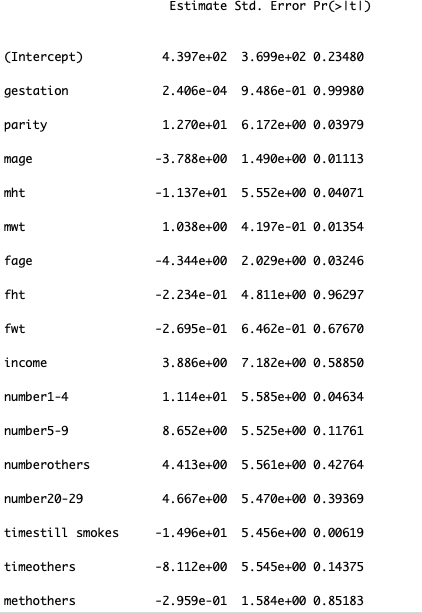
\includegraphics{/Users/gengyaoyuan/Desktop/123/1.png}\\
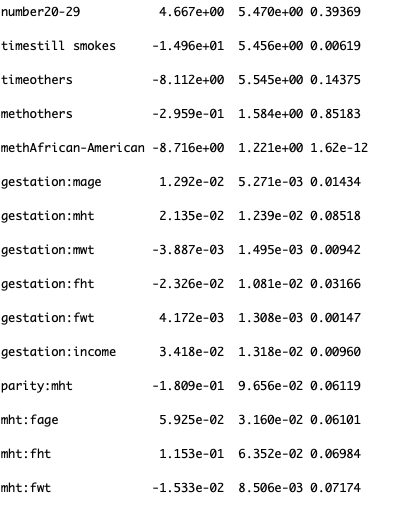
\includegraphics{/Users/gengyaoyuan/Desktop/123/2.png}\\
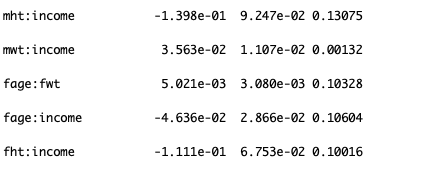
\includegraphics{/Users/gengyaoyuan/Desktop/123/3.png}

\section{Discussion}\subsection{What are the most important factors associated with/influencing birth weight?}

According to the summary of m1, the most important factors are the
`total number of previous pregnancies,' `African-American mother,' `the
father's weight,' `the mother's weight,' `smoke time' and many
interactions between `gestation' with the previous factors. Simply, it
seems like the length of gestation, the number of pregnancies times,
ethnicity of mother, mother smoke or not and the weight of parents are
the most critical factors.
\subsection{Low birth weight is considered to be 88 ounces or less. Based on this analysis, would you be able to recommend behavioral changes to parents in order to avoid low birthweight? If so, please carefully formulate your recommendation.}

\subsection{Are there any coecients with high p-values retained in the final model? If so, why?}

YES, the p-value of `the length of the gestation period' is high,
however, its interactions with a total number of previous
pregnancies,`'African-American mother,' `the father???s weight,' and
`the mother???s weight,' all has tiny p-values close to 0. This is
because `the length of the gestation period' itself is not important,
but its interactions with others are so important for the model.

\textbackslash{}subsection\{Are there any outlying observations that
might be appropriate to remove?

From the fitted values vs.~residual values graph in 2.6.3, our final
graph is the graph three, since the fitted values are not following any
linear relationship, all points are crowded together is acceptable for
us. By the definition of outliers, which the points with particular
residual means outliers, yes, there are some observations that we need
to remove. It is also the same for leverage points for the graph in
2.6.4's boxplot; there are some points with outstanding x, they are
leverage points that needed to remove. Since the 2.6.3 graph shows
almost all fitted variables follow a line, we can get a conclusion that
there is no important variables need to remove.

\subsection{Are any of the regression assumptions of the final model violated? If so, which ones?}

At first we assume `'the length of the gestation period', `income' and
`the age' and 'height of parents'are important factors, but basing on
the too large p-value, we drop them as last.

\subsection{What are the possible deficiencies of the final model?   how do these deficienciesnuance your conclusions/recommendations above?}

Since there are too many NA data in `The mother???s height' and `the
total number of previous pregnancies'(over 35\%), these NA datapoints
may cause serious bias on our model. We try to fix these data points by
using MICE founction, if the data of `The mother???s height' and `the
total number of previous pregnancies' follow normal distribution(the
help distribution used in MICE fouction), our prediction will close to
original data, otherwise our model will contain some bias.

\section{Appendix}

\begin{Shaded}
\begin{Highlighting}[]
\KeywordTok{library}\NormalTok{(mice)}

\CommentTok{# data input }
\NormalTok{chds_births <-}\StringTok{ }\KeywordTok{read.csv}\NormalTok{(}\DataTypeTok{file =} \StringTok{"chds_births.csv"}\NormalTok{)}
\KeywordTok{summary}\NormalTok{(chds_births) }\CommentTok{# first look of the data}
\end{Highlighting}
\end{Shaded}

\begin{verbatim}
##        wt          gestation         parity            meth       
##  Min.   : 55.0   Min.   :148.0   Min.   : 0.000   Min.   : 0.000  
##  1st Qu.:108.8   1st Qu.:272.0   1st Qu.: 0.000   1st Qu.: 0.000  
##  Median :120.0   Median :280.0   Median : 1.000   Median : 3.000  
##  Mean   :119.6   Mean   :279.3   Mean   : 1.932   Mean   : 3.129  
##  3rd Qu.:131.0   3rd Qu.:288.0   3rd Qu.: 3.000   3rd Qu.: 7.000  
##  Max.   :176.0   Max.   :353.0   Max.   :13.000   Max.   :10.000  
##                  NA's   :13                       NA's   :1       
##       mage            med             mht             mwt       
##  Min.   :15.00   Min.   :0.000   Min.   :53.00   Min.   : 87.0  
##  1st Qu.:23.00   1st Qu.:2.000   1st Qu.:62.00   1st Qu.:114.8  
##  Median :26.00   Median :2.000   Median :64.00   Median :125.0  
##  Mean   :27.26   Mean   :2.917   Mean   :64.05   Mean   :128.6  
##  3rd Qu.:31.00   3rd Qu.:4.000   3rd Qu.:66.00   3rd Qu.:139.0  
##  Max.   :45.00   Max.   :7.000   Max.   :72.00   Max.   :250.0  
##  NA's   :2       NA's   :1       NA's   :22      NA's   :36     
##       feth             fage            fed             fht      
##  Min.   : 0.000   Min.   :18.00   Min.   :0.000   Min.   :60.0  
##  1st Qu.: 0.000   1st Qu.:25.00   1st Qu.:2.000   1st Qu.:68.0  
##  Median : 3.000   Median :29.00   Median :4.000   Median :71.0  
##  Mean   : 3.154   Mean   :30.35   Mean   :3.127   Mean   :70.2  
##  3rd Qu.: 7.000   3rd Qu.:34.00   3rd Qu.:5.000   3rd Qu.:72.0  
##  Max.   :10.000   Max.   :62.00   Max.   :7.000   Max.   :78.0  
##  NA's   :31       NA's   :7       NA's   :13      NA's   :492   
##       fwt           marital          income          smoke       
##  Min.   :110.0   Min.   :0.000   Min.   :0.000   Min.   :0.0000  
##  1st Qu.:155.0   1st Qu.:1.000   1st Qu.:2.000   1st Qu.:0.0000  
##  Median :170.0   Median :1.000   Median :3.000   Median :1.0000  
##  Mean   :171.2   Mean   :1.038   Mean   :3.701   Mean   :0.8018  
##  3rd Qu.:185.0   3rd Qu.:1.000   3rd Qu.:5.000   3rd Qu.:1.0000  
##  Max.   :260.0   Max.   :5.000   Max.   :9.000   Max.   :3.0000  
##  NA's   :499                     NA's   :124     NA's   :10      
##       time            number    
##  Min.   :0.0000   Min.   :0.00  
##  1st Qu.:0.0000   1st Qu.:0.00  
##  Median :1.0000   Median :1.00  
##  Mean   :0.9625   Mean   :1.76  
##  3rd Qu.:1.0000   3rd Qu.:3.00  
##  Max.   :9.0000   Max.   :8.00  
##  NA's   :10       NA's   :21
\end{verbatim}

\begin{Shaded}
\begin{Highlighting}[]
\CommentTok{# standardize the category variable marital}
\NormalTok{chds_births}\OperatorTok{$}\NormalTok{marital[}\OperatorTok{!}\NormalTok{chds_births}\OperatorTok{$}\NormalTok{marital }\OperatorTok\StringTok{ }\KeywordTok{c}\NormalTok{(}\DecValTok{1}\OperatorTok{:}\DecValTok{5}\NormalTok{)] =}\StringTok{ }\OtherTok{NA}

\CommentTok{# standardize the category variable meth}
\NormalTok{chds_births}\OperatorTok{$}\NormalTok{meth[chds_births}\OperatorTok{$}\NormalTok{meth }\OperatorTok\StringTok{ }\KeywordTok{c}\NormalTok{(}\DecValTok{0}\NormalTok{,}\DecValTok{1}\NormalTok{,}\DecValTok{2}\NormalTok{,}\DecValTok{3}\NormalTok{,}\DecValTok{4}\NormalTok{,}\DecValTok{5}\NormalTok{)] =}\StringTok{ }\DecValTok{0}
\NormalTok{chds_births}\OperatorTok{$}\NormalTok{meth[chds_births}\OperatorTok{$}\NormalTok{meth }\OperatorTok\StringTok{ }\KeywordTok{c}\NormalTok{(}\DecValTok{6}\NormalTok{)] =}\StringTok{ }\DecValTok{1}
\NormalTok{chds_births}\OperatorTok{$}\NormalTok{meth[chds_births}\OperatorTok{$}\NormalTok{meth }\OperatorTok\StringTok{ }\KeywordTok{c}\NormalTok{(}\DecValTok{7}\NormalTok{)] =}\StringTok{ }\DecValTok{2}
\NormalTok{chds_births}\OperatorTok{$}\NormalTok{meth[chds_births}\OperatorTok{$}\NormalTok{meth }\OperatorTok\StringTok{ }\KeywordTok{c}\NormalTok{(}\DecValTok{8}\NormalTok{)] =}\StringTok{ }\DecValTok{3}
\NormalTok{chds_births}\OperatorTok{$}\NormalTok{meth[chds_births}\OperatorTok{$}\NormalTok{meth }\OperatorTok\StringTok{ }\KeywordTok{c}\NormalTok{(}\DecValTok{9}\NormalTok{)] =}\StringTok{ }\DecValTok{4}
\NormalTok{chds_births}\OperatorTok{$}\NormalTok{meth[chds_births}\OperatorTok{$}\NormalTok{meth }\OperatorTok\StringTok{ }\KeywordTok{c}\NormalTok{(}\DecValTok{10}\NormalTok{)] =}\StringTok{ }\DecValTok{5}

\CommentTok{# standardize the category variable feth}
\NormalTok{chds_births}\OperatorTok{$}\NormalTok{feth[chds_births}\OperatorTok{$}\NormalTok{feth }\OperatorTok\StringTok{ }\KeywordTok{c}\NormalTok{(}\DecValTok{0}\NormalTok{,}\DecValTok{1}\NormalTok{,}\DecValTok{2}\NormalTok{,}\DecValTok{3}\NormalTok{,}\DecValTok{4}\NormalTok{,}\DecValTok{5}\NormalTok{)] =}\StringTok{ }\DecValTok{0}
\NormalTok{chds_births}\OperatorTok{$}\NormalTok{feth[chds_births}\OperatorTok{$}\NormalTok{feth }\OperatorTok\StringTok{ }\KeywordTok{c}\NormalTok{(}\DecValTok{6}\NormalTok{)] =}\StringTok{ }\DecValTok{1}
\NormalTok{chds_births}\OperatorTok{$}\NormalTok{feth[chds_births}\OperatorTok{$}\NormalTok{feth }\OperatorTok\StringTok{ }\KeywordTok{c}\NormalTok{(}\DecValTok{7}\NormalTok{)] =}\StringTok{ }\DecValTok{2}
\NormalTok{chds_births}\OperatorTok{$}\NormalTok{feth[chds_births}\OperatorTok{$}\NormalTok{feth }\OperatorTok\StringTok{ }\KeywordTok{c}\NormalTok{(}\DecValTok{8}\NormalTok{)] =}\StringTok{ }\DecValTok{3}
\NormalTok{chds_births}\OperatorTok{$}\NormalTok{feth[chds_births}\OperatorTok{$}\NormalTok{feth }\OperatorTok\StringTok{ }\KeywordTok{c}\NormalTok{(}\DecValTok{9}\NormalTok{)] =}\StringTok{ }\DecValTok{4}
\NormalTok{chds_births}\OperatorTok{$}\NormalTok{feth[chds_births}\OperatorTok{$}\NormalTok{feth }\OperatorTok\StringTok{ }\KeywordTok{c}\NormalTok{(}\DecValTok{10}\NormalTok{)] =}\StringTok{ }\DecValTok{5}

\CommentTok{# change all category variables to factor instead of continues variables}
\NormalTok{chds_births}\OperatorTok{$}\NormalTok{meth <-}\StringTok{ }\KeywordTok{as.factor}\NormalTok{(chds_births}\OperatorTok{$}\NormalTok{meth)}
\NormalTok{chds_births}\OperatorTok{$}\NormalTok{med <-}\StringTok{ }\KeywordTok{as.factor}\NormalTok{(chds_births}\OperatorTok{$}\NormalTok{med)}
\NormalTok{chds_births}\OperatorTok{$}\NormalTok{feth <-}\StringTok{ }\KeywordTok{as.factor}\NormalTok{(chds_births}\OperatorTok{$}\NormalTok{feth)}
\NormalTok{chds_births}\OperatorTok{$}\NormalTok{fed <-}\StringTok{ }\KeywordTok{as.factor}\NormalTok{(chds_births}\OperatorTok{$}\NormalTok{fed)}
\NormalTok{chds_births}\OperatorTok{$}\NormalTok{marital <-}\StringTok{ }\KeywordTok{as.factor}\NormalTok{(chds_births}\OperatorTok{$}\NormalTok{marital)}
\NormalTok{chds_births}\OperatorTok{$}\NormalTok{smoke <-}\StringTok{ }\KeywordTok{as.factor}\NormalTok{(chds_births}\OperatorTok{$}\NormalTok{smoke)}
\NormalTok{chds_births}\OperatorTok{$}\NormalTok{time <-}\StringTok{ }\KeywordTok{as.factor}\NormalTok{(chds_births}\OperatorTok{$}\NormalTok{time)}
\NormalTok{chds_births}\OperatorTok{$}\NormalTok{number <-}\StringTok{ }\KeywordTok{as.factor}\NormalTok{(chds_births}\OperatorTok{$}\NormalTok{number)}

\CommentTok{# remove the NA by mice which method is sample}
\NormalTok{births_mice <-}\StringTok{ }\KeywordTok{mice}\NormalTok{(chds_births, }\DataTypeTok{method =} \StringTok{"sample"}\NormalTok{, }\DataTypeTok{seed =} \DecValTok{1}\NormalTok{)}
\end{Highlighting}
\end{Shaded}

\begin{verbatim}
## 
##  iter imp variable
##   1   1  gestation  meth  mage  med  mht  mwt  feth  fage  fed  fht  fwt  marital  income  smoke  time  number
##   1   2  gestation  meth  mage  med  mht  mwt  feth  fage  fed  fht  fwt  marital  income  smoke  time  number
##   1   3  gestation  meth  mage  med  mht  mwt  feth  fage  fed  fht  fwt  marital  income  smoke  time  number
##   1   4  gestation  meth  mage  med  mht  mwt  feth  fage  fed  fht  fwt  marital  income  smoke  time  number
##   1   5  gestation  meth  mage  med  mht  mwt  feth  fage  fed  fht  fwt  marital  income  smoke  time  number
##   2   1  gestation  meth  mage  med  mht  mwt  feth  fage  fed  fht  fwt  marital  income  smoke  time  number
##   2   2  gestation  meth  mage  med  mht  mwt  feth  fage  fed  fht  fwt  marital  income  smoke  time  number
##   2   3  gestation  meth  mage  med  mht  mwt  feth  fage  fed  fht  fwt  marital  income  smoke  time  number
##   2   4  gestation  meth  mage  med  mht  mwt  feth  fage  fed  fht  fwt  marital  income  smoke  time  number
##   2   5  gestation  meth  mage  med  mht  mwt  feth  fage  fed  fht  fwt  marital  income  smoke  time  number
##   3   1  gestation  meth  mage  med  mht  mwt  feth  fage  fed  fht  fwt  marital  income  smoke  time  number
##   3   2  gestation  meth  mage  med  mht  mwt  feth  fage  fed  fht  fwt  marital  income  smoke  time  number
##   3   3  gestation  meth  mage  med  mht  mwt  feth  fage  fed  fht  fwt  marital  income  smoke  time  number
##   3   4  gestation  meth  mage  med  mht  mwt  feth  fage  fed  fht  fwt  marital  income  smoke  time  number
##   3   5  gestation  meth  mage  med  mht  mwt  feth  fage  fed  fht  fwt  marital  income  smoke  time  number
##   4   1  gestation  meth  mage  med  mht  mwt  feth  fage  fed  fht  fwt  marital  income  smoke  time  number
##   4   2  gestation  meth  mage  med  mht  mwt  feth  fage  fed  fht  fwt  marital  income  smoke  time  number
##   4   3  gestation  meth  mage  med  mht  mwt  feth  fage  fed  fht  fwt  marital  income  smoke  time  number
##   4   4  gestation  meth  mage  med  mht  mwt  feth  fage  fed  fht  fwt  marital  income  smoke  time  number
##   4   5  gestation  meth  mage  med  mht  mwt  feth  fage  fed  fht  fwt  marital  income  smoke  time  number
##   5   1  gestation  meth  mage  med  mht  mwt  feth  fage  fed  fht  fwt  marital  income  smoke  time  number
##   5   2  gestation  meth  mage  med  mht  mwt  feth  fage  fed  fht  fwt  marital  income  smoke  time  number
##   5   3  gestation  meth  mage  med  mht  mwt  feth  fage  fed  fht  fwt  marital  income  smoke  time  number
##   5   4  gestation  meth  mage  med  mht  mwt  feth  fage  fed  fht  fwt  marital  income  smoke  time  number
##   5   5  gestation  meth  mage  med  mht  mwt  feth  fage  fed  fht  fwt  marital  income  smoke  time  number
\end{verbatim}

\begin{verbatim}
## Warning: Number of logged events: 160
\end{verbatim}

\begin{Shaded}
\begin{Highlighting}[]
\NormalTok{births_clean <-}\StringTok{ }\KeywordTok{complete}\NormalTok{(births_mice)}

\KeywordTok{anyNA}\NormalTok{(births_clean) }\CommentTok{#check the NA after removement}
\end{Highlighting}
\end{Shaded}

\begin{verbatim}
## [1] FALSE
\end{verbatim}

\begin{Shaded}
\begin{Highlighting}[]
 \CommentTok{# since we operate by levels of the factor, for }
 \CommentTok{# factor '0' it will be position '1' in levels}

\CommentTok{# category variable: meth}
\KeywordTok{levels}\NormalTok{(births_clean}\OperatorTok{$}\NormalTok{meth)}
\end{Highlighting}
\end{Shaded}

\begin{verbatim}
## [1] "0" "1" "2" "3" "4" "5"
\end{verbatim}

\begin{Shaded}
\begin{Highlighting}[]
\KeywordTok{levels}\NormalTok{(births_clean}\OperatorTok{$}\NormalTok{meth)[}\DecValTok{1}\NormalTok{] <-}\StringTok{ "Caucasian"}
\KeywordTok{levels}\NormalTok{(births_clean}\OperatorTok{$}\NormalTok{meth)[}\DecValTok{3}\NormalTok{] <-}\StringTok{ "African-American"}
\KeywordTok{levels}\NormalTok{(births_clean}\OperatorTok{$}\NormalTok{meth)[}\KeywordTok{c}\NormalTok{(}\DecValTok{2}\NormalTok{,}\DecValTok{4}\NormalTok{,}\DecValTok{5}\NormalTok{,}\DecValTok{6}\NormalTok{)]<-}\StringTok{ "others"}

\CommentTok{# category variable: med}
\KeywordTok{levels}\NormalTok{(births_clean}\OperatorTok{$}\NormalTok{med)[}\DecValTok{2}\NormalTok{] <-}\StringTok{ "middle-school"}
\KeywordTok{levels}\NormalTok{(births_clean}\OperatorTok{$}\NormalTok{med)[}\DecValTok{3}\NormalTok{] <-}\StringTok{ "high-school"}
\KeywordTok{levels}\NormalTok{(births_clean}\OperatorTok{$}\NormalTok{med)[}\DecValTok{5}\NormalTok{] <-}\StringTok{ "high-school + some college"}
\KeywordTok{levels}\NormalTok{(births_clean}\OperatorTok{$}\NormalTok{med)[}\DecValTok{6}\NormalTok{] <-}\StringTok{ "college graduate"}
\KeywordTok{levels}\NormalTok{(births_clean}\OperatorTok{$}\NormalTok{med)[}\KeywordTok{c}\NormalTok{(}\DecValTok{1}\NormalTok{,}\DecValTok{4}\NormalTok{,}\DecValTok{7}\NormalTok{,}\DecValTok{8}\NormalTok{)]<-}\StringTok{ "others"}

\CommentTok{# category variable: feth}
\KeywordTok{levels}\NormalTok{(births_clean}\OperatorTok{$}\NormalTok{feth)}
\end{Highlighting}
\end{Shaded}

\begin{verbatim}
## [1] "0" "1" "2" "3" "4" "5"
\end{verbatim}

\begin{Shaded}
\begin{Highlighting}[]
\KeywordTok{levels}\NormalTok{(births_clean}\OperatorTok{$}\NormalTok{feth)[}\DecValTok{1}\NormalTok{] <-}\StringTok{ "Caucasian"}
\KeywordTok{levels}\NormalTok{(births_clean}\OperatorTok{$}\NormalTok{feth)[}\DecValTok{3}\NormalTok{] <-}\StringTok{ "African-American"}
\KeywordTok{levels}\NormalTok{(births_clean}\OperatorTok{$}\NormalTok{feth)[}\KeywordTok{c}\NormalTok{(}\DecValTok{2}\NormalTok{,}\DecValTok{4}\NormalTok{,}\DecValTok{5}\NormalTok{,}\DecValTok{6}\NormalTok{)]<-}\StringTok{ "others"}

\CommentTok{# category variable: fed}
\KeywordTok{levels}\NormalTok{(births_clean}\OperatorTok{$}\NormalTok{fed)[}\DecValTok{2}\NormalTok{] <-}\StringTok{ "middle-school"}
\KeywordTok{levels}\NormalTok{(births_clean}\OperatorTok{$}\NormalTok{fed)[}\DecValTok{3}\NormalTok{] <-}\StringTok{ "high-school"}
\KeywordTok{levels}\NormalTok{(births_clean}\OperatorTok{$}\NormalTok{fed)[}\DecValTok{5}\NormalTok{] <-}\StringTok{ "high-school + some college"}
\KeywordTok{levels}\NormalTok{(births_clean}\OperatorTok{$}\NormalTok{fed)[}\DecValTok{6}\NormalTok{] <-}\StringTok{ "college graduate"}
\KeywordTok{levels}\NormalTok{(births_clean}\OperatorTok{$}\NormalTok{fed)[}\KeywordTok{c}\NormalTok{(}\DecValTok{1}\NormalTok{,}\DecValTok{4}\NormalTok{,}\DecValTok{7}\NormalTok{,}\DecValTok{8}\NormalTok{)]<-}\StringTok{ "others"}

\CommentTok{# category variable: marital}
\KeywordTok{levels}\NormalTok{(births_clean}\OperatorTok{$}\NormalTok{marital)[}\DecValTok{1}\NormalTok{] <-}\StringTok{ "married"}
\KeywordTok{levels}\NormalTok{(births_clean}\OperatorTok{$}\NormalTok{marital)[}\KeywordTok{c}\NormalTok{(}\DecValTok{2}\NormalTok{,}\DecValTok{3}\NormalTok{,}\DecValTok{4}\NormalTok{,}\DecValTok{5}\NormalTok{)] <-}\StringTok{ "others"}

\CommentTok{# delete smoke }
\NormalTok{births_clean}\OperatorTok{$}\NormalTok{smoke =}\StringTok{ }\OtherTok{NULL}

\CommentTok{# category variable: time}
\KeywordTok{levels}\NormalTok{(births_clean}\OperatorTok{$}\NormalTok{time)[}\DecValTok{1}\NormalTok{] <-}\StringTok{ "never smoked"}
\KeywordTok{levels}\NormalTok{(births_clean}\OperatorTok{$}\NormalTok{time)[}\DecValTok{2}\NormalTok{] <-}\StringTok{ "still smokes"}
\KeywordTok{levels}\NormalTok{(births_clean}\OperatorTok{$}\NormalTok{time)[}\KeywordTok{c}\NormalTok{(}\DecValTok{3}\NormalTok{,}\DecValTok{4}\NormalTok{,}\DecValTok{5}\NormalTok{,}\DecValTok{6}\NormalTok{,}\DecValTok{7}\NormalTok{,}\DecValTok{8}\NormalTok{,}\DecValTok{9}\NormalTok{,}\DecValTok{10}\NormalTok{)] <-}\StringTok{ "others"}

\CommentTok{# category variable: number}
\KeywordTok{levels}\NormalTok{(births_clean}\OperatorTok{$}\NormalTok{number)[}\DecValTok{1}\NormalTok{] <-}\StringTok{ "never smoked"}
\KeywordTok{levels}\NormalTok{(births_clean}\OperatorTok{$}\NormalTok{number)[}\DecValTok{2}\NormalTok{] <-}\StringTok{ "1-4"}
\KeywordTok{levels}\NormalTok{(births_clean}\OperatorTok{$}\NormalTok{number)[}\DecValTok{3}\NormalTok{] <-}\StringTok{ "5-9"}
\KeywordTok{levels}\NormalTok{(births_clean}\OperatorTok{$}\NormalTok{number)[}\DecValTok{6}\NormalTok{] <-}\StringTok{ "20-29"}
\KeywordTok{levels}\NormalTok{(births_clean}\OperatorTok{$}\NormalTok{number)[}\KeywordTok{c}\NormalTok{(}\DecValTok{4}\NormalTok{,}\DecValTok{5}\NormalTok{,}\DecValTok{7}\NormalTok{,}\DecValTok{8}\NormalTok{,}\DecValTok{9}\NormalTok{,}\DecValTok{10}\NormalTok{)] <-}\StringTok{ "others"}

\CommentTok{#summary of new data}
\KeywordTok{summary}\NormalTok{(births_clean)}
\end{Highlighting}
\end{Shaded}

\begin{verbatim}
##        wt          gestation         parity                     meth    
##  Min.   : 55.0   Min.   :148.0   Min.   : 0.000   Caucasian       :871  
##  1st Qu.:108.8   1st Qu.:272.0   1st Qu.: 0.000   others          :121  
##  Median :120.0   Median :280.0   Median : 1.000   African-American:244  
##  Mean   :119.6   Mean   :279.3   Mean   : 1.932                         
##  3rd Qu.:131.0   3rd Qu.:288.0   3rd Qu.: 3.000                         
##  Max.   :176.0   Max.   :353.0   Max.   :13.000                         
##       mage                               med           mht       
##  Min.   :15.00   others                    : 91   Min.   :53.00  
##  1st Qu.:23.00   middle-school             :183   1st Qu.:62.00  
##  Median :26.00   high-school               :444   Median :64.00  
##  Mean   :27.25   high-school + some college:299   Mean   :64.04  
##  3rd Qu.:31.00   college graduate          :219   3rd Qu.:66.00  
##  Max.   :45.00                                    Max.   :72.00  
##       mwt                      feth          fage      
##  Min.   : 87.0   Caucasian       :881   Min.   :18.00  
##  1st Qu.:114.0   others          : 97   1st Qu.:25.00  
##  Median :125.0   African-American:258   Median :29.00  
##  Mean   :128.6                          Mean   :30.35  
##  3rd Qu.:139.0                          3rd Qu.:34.00  
##  Max.   :250.0                          Max.   :62.00  
##                          fed           fht             fwt       
##  others                    : 78   Min.   :60.00   Min.   :110.0  
##  middle-school             :195   1st Qu.:68.00   1st Qu.:155.0  
##  high-school               :345   Median :71.00   Median :170.0  
##  high-school + some college:268   Mean   :70.23   Mean   :170.9  
##  college graduate          :350   3rd Qu.:72.00   3rd Qu.:185.0  
##                                   Max.   :78.00   Max.   :260.0  
##     marital         income                time              number   
##  married:1210   Min.   :0.000   never smoked:548   never smoked:550  
##  others :  26   1st Qu.:2.000   still smokes:489   1-4         :160  
##                 Median :3.000   others      :199   5-9         :168  
##                 Mean   :3.667                      others      :157  
##                 3rd Qu.:5.000                      20-29       :201  
##                 Max.   :9.000
\end{verbatim}

\begin{Shaded}
\begin{Highlighting}[]
\CommentTok{# pairplot for continues data}
\KeywordTok{pairs}\NormalTok{(}\OperatorTok{~}\NormalTok{wt }\OperatorTok{+}\StringTok{ }\NormalTok{gestation }\OperatorTok{+}\StringTok{ }\NormalTok{parity }\OperatorTok{+}\StringTok{ }\NormalTok{mage }\OperatorTok{+}\StringTok{ }\NormalTok{mht }\OperatorTok{+}\StringTok{ }\NormalTok{mwt }\OperatorTok{+}\StringTok{ }\NormalTok{fage }\OperatorTok{+}\StringTok{ }\NormalTok{fht }\OperatorTok{+}\StringTok{ }\NormalTok{fwt,}\DataTypeTok{cex =}\NormalTok{ .}\DecValTok{05}\NormalTok{,  }\DataTypeTok{data =}\NormalTok{ chds_births)}
\end{Highlighting}
\end{Shaded}

\includegraphics{331finalproject_files/figure-latex/unnamed-chunk-26-1.pdf}

\begin{Shaded}
\begin{Highlighting}[]
\KeywordTok{pairs}\NormalTok{(}\OperatorTok{~}\NormalTok{wt }\OperatorTok{+}\StringTok{ }\NormalTok{gestation }\OperatorTok{+}\StringTok{ }\NormalTok{mage }\OperatorTok{+}\StringTok{ }\NormalTok{mwt }\OperatorTok{+}\StringTok{ }\NormalTok{fage }\OperatorTok{+}\StringTok{ }\NormalTok{fwt,}\DataTypeTok{cex =}\NormalTok{ .}\DecValTok{05}\NormalTok{,  }\DataTypeTok{data =}\NormalTok{ chds_births) }\CommentTok{# detailed pairplots}
\end{Highlighting}
\end{Shaded}

\includegraphics{331finalproject_files/figure-latex/unnamed-chunk-26-2.pdf}

\begin{Shaded}
\begin{Highlighting}[]
\NormalTok{M0 <-}\StringTok{ }\KeywordTok{lm}\NormalTok{(wt }\OperatorTok{~}\StringTok{ }\DecValTok{1}\NormalTok{, }\DataTypeTok{data =}\NormalTok{ births_clean) }\CommentTok{# initial model}
\NormalTok{Mmax <-}\StringTok{ }\KeywordTok{lm}\NormalTok{(wt }\OperatorTok{~}\StringTok{ }\NormalTok{(.)}\OperatorTok{^}\DecValTok{2}\NormalTok{ , }\DataTypeTok{data =}\NormalTok{ births_clean) }\CommentTok{# full model}
\NormalTok{Mstart <-}\StringTok{ }\KeywordTok{lm}\NormalTok{(wt }\OperatorTok{~}\StringTok{ }\NormalTok{., }\DataTypeTok{data =}\NormalTok{ births_clean) }\CommentTok{#start model}

\CommentTok{# detect coefficients which are NAs}
\NormalTok{beta.max <-}\StringTok{ }\KeywordTok{coef}\NormalTok{(Mmax)}
\KeywordTok{names}\NormalTok{(beta.max)[}\KeywordTok{is.na}\NormalTok{(beta.max)]}
\end{Highlighting}
\end{Shaded}

\begin{verbatim}
##  [1] "medhigh-school + some college:number20-29"
##  [2] "medcollege graduate:number20-29"          
##  [3] "mht:number20-29"                          
##  [4] "mwt:number20-29"                          
##  [5] "fethAfrican-American:maritalothers"       
##  [6] "fethothers:number20-29"                   
##  [7] "fethAfrican-American:number20-29"         
##  [8] "fage:number20-29"                         
##  [9] "fedcollege graduate:maritalothers"        
## [10] "fedmiddle-school:number20-29"             
## [11] "fedhigh-school:number20-29"               
## [12] "fedhigh-school + some college:number20-29"
## [13] "fedcollege graduate:number20-29"          
## [14] "fht:number20-29"                          
## [15] "fwt:number20-29"                          
## [16] "maritalothers:number1-4"                  
## [17] "maritalothers:number20-29"                
## [18] "income:number20-29"                       
## [19] "timeothers:number1-4"                     
## [20] "timeothers:number5-9"                     
## [21] "timeothers:numberothers"                  
## [22] "timestill smokes:number20-29"             
## [23] "timeothers:number20-29"
\end{verbatim}

\begin{Shaded}
\begin{Highlighting}[]
\KeywordTok{anyNA}\NormalTok{(}\KeywordTok{coef}\NormalTok{(Mmax))}
\end{Highlighting}
\end{Shaded}

\begin{verbatim}
## [1] TRUE
\end{verbatim}

\begin{Shaded}
\begin{Highlighting}[]
\NormalTok{Mmax <-}\StringTok{ }\KeywordTok{lm}\NormalTok{(wt }\OperatorTok{~}\StringTok{ }\NormalTok{(. }\OperatorTok{-}\NormalTok{marital }\OperatorTok{-}\NormalTok{fed }\OperatorTok{-}\NormalTok{feth }\OperatorTok{-}\NormalTok{number }\OperatorTok{-}\NormalTok{time }\OperatorTok{-}\StringTok{ }\NormalTok{meth }\OperatorTok{-}\NormalTok{med)}\OperatorTok{^}\DecValTok{2} 
           \OperatorTok{+}\NormalTok{marital }\OperatorTok{+}\StringTok{ }\NormalTok{fed }\OperatorTok{+}\NormalTok{feth }\OperatorTok{+}\NormalTok{number }\OperatorTok{+}\NormalTok{time }\OperatorTok{+}\StringTok{ }\NormalTok{meth }\OperatorTok{+}\NormalTok{med , }\DataTypeTok{data =}\NormalTok{ births_clean) }\CommentTok{# Revised max model}
\NormalTok{Mstart <-}\StringTok{ }\KeywordTok{lm}\NormalTok{(wt }\OperatorTok{~}\StringTok{ }\NormalTok{., }\DataTypeTok{data =}\NormalTok{ births_clean) }\CommentTok{#start model}
\KeywordTok{anyNA}\NormalTok{(}\KeywordTok{coef}\NormalTok{(Mmax)) }\CommentTok{# detect coefficients which are NAs}
\end{Highlighting}
\end{Shaded}

\begin{verbatim}
## [1] FALSE
\end{verbatim}

\begin{Shaded}
\begin{Highlighting}[]
\CommentTok{# Forward selection}
\KeywordTok{invisible}\NormalTok{(Mfwd <-}\StringTok{ }\KeywordTok{step}\NormalTok{(}\DataTypeTok{object =}\NormalTok{ M0,}
               \DataTypeTok{scope =} \KeywordTok{list}\NormalTok{(}\DataTypeTok{lower =}\NormalTok{ M0, }\DataTypeTok{upper =}\NormalTok{ Mmax),}
               \DataTypeTok{direction =} \StringTok{"forward"}\NormalTok{, }\DataTypeTok{trace =} \OtherTok{FALSE}\NormalTok{))}

\CommentTok{# Backward elimination selection}
\NormalTok{Mback <-}\StringTok{ }\KeywordTok{step}\NormalTok{(}\DataTypeTok{object =}\NormalTok{ Mmax, }
              \DataTypeTok{scope =} \KeywordTok{list}\NormalTok{(}\DataTypeTok{lower =}\NormalTok{ M0, }\DataTypeTok{upper =}\NormalTok{ Mmax),}
              \DataTypeTok{direction =} \StringTok{"backward"}\NormalTok{, }\DataTypeTok{trace =} \OtherTok{FALSE}\NormalTok{)}

\CommentTok{# Stepwise selection}
\NormalTok{Mstep <-}\StringTok{ }\KeywordTok{step}\NormalTok{(}\DataTypeTok{object =}\NormalTok{ Mstart,}
              \DataTypeTok{scope =} \KeywordTok{list}\NormalTok{(}\DataTypeTok{lower =}\NormalTok{ M0, }\DataTypeTok{upper =}\NormalTok{ Mmax),}
              \DataTypeTok{direction =} \StringTok{"both"}\NormalTok{, }\DataTypeTok{trace =} \OtherTok{FALSE}\NormalTok{)}

\KeywordTok{c}\NormalTok{(}\DataTypeTok{fwd =} \KeywordTok{length}\NormalTok{(}\KeywordTok{coef}\NormalTok{(Mfwd)), }\DataTypeTok{back =} \KeywordTok{length}\NormalTok{(}\KeywordTok{coef}\NormalTok{(Mback)), }\DataTypeTok{step =} \KeywordTok{length}\NormalTok{(}\KeywordTok{coef}\NormalTok{(Mstep)))}
\end{Highlighting}
\end{Shaded}

\begin{verbatim}
##  fwd back step 
##   20   33   25
\end{verbatim}

\begin{Shaded}
\begin{Highlighting}[]
\NormalTok{Mfwd}\OperatorTok{$}\NormalTok{call}
\end{Highlighting}
\end{Shaded}

\begin{verbatim}
## lm(formula = wt ~ gestation + time + mht + meth + parity + number + 
##     fwt + mwt + fht + gestation:fwt + gestation:mwt + mht:fwt + 
##     gestation:mht + gestation:fht, data = births_clean)
\end{verbatim}

\begin{Shaded}
\begin{Highlighting}[]
\NormalTok{Mback}\OperatorTok{$}\NormalTok{call}
\end{Highlighting}
\end{Shaded}

\begin{verbatim}
## lm(formula = wt ~ gestation + parity + mage + mht + mwt + fage + 
##     fht + fwt + income + number + time + meth + gestation:mage + 
##     gestation:mht + gestation:mwt + gestation:fht + gestation:fwt + 
##     gestation:income + parity:mht + mht:fage + mht:fht + mht:fwt + 
##     mht:income + mwt:income + fage:fwt + fage:income + fht:income, 
##     data = births_clean)
\end{verbatim}

\begin{Shaded}
\begin{Highlighting}[]
\NormalTok{Mstep}\OperatorTok{$}\NormalTok{call}
\end{Highlighting}
\end{Shaded}

\begin{verbatim}
## lm(formula = wt ~ gestation + parity + meth + mage + mht + mwt + 
##     fht + fwt + income + time + number + gestation:income + mwt:income + 
##     gestation:mage + gestation:fwt + gestation:mwt + gestation:fht + 
##     gestation:mht + fht:income, data = births_clean)
\end{verbatim}

\begin{Shaded}
\begin{Highlighting}[]
\KeywordTok{par}\NormalTok{(}\DataTypeTok{mfrow=}\KeywordTok{c}\NormalTok{(}\DecValTok{2}\NormalTok{,}\DecValTok{3}\NormalTok{))}
\KeywordTok{plot}\NormalTok{(}\KeywordTok{fitted}\NormalTok{(Mfwd), }\KeywordTok{residuals}\NormalTok{(Mfwd), }\DataTypeTok{main=}\StringTok{"forward"}\NormalTok{, }\DataTypeTok{cex =}\NormalTok{ .}\DecValTok{2}\NormalTok{)}
\KeywordTok{plot}\NormalTok{(}\KeywordTok{fitted}\NormalTok{(Mback), }\KeywordTok{residuals}\NormalTok{(Mback), }\DataTypeTok{main=}\StringTok{"backward"}\NormalTok{, }\DataTypeTok{cex =}\NormalTok{ .}\DecValTok{2}\NormalTok{)}
\KeywordTok{plot}\NormalTok{(}\KeywordTok{fitted}\NormalTok{(Mstep), }\KeywordTok{residuals}\NormalTok{(Mstep), }\DataTypeTok{main=}\StringTok{"stepwise"}\NormalTok{, }\DataTypeTok{cex =}\NormalTok{.}\DecValTok{2}\NormalTok{)}
\KeywordTok{qqnorm}\NormalTok{(}\KeywordTok{residuals}\NormalTok{(Mfwd), }\DataTypeTok{main=}\StringTok{"forward"}\NormalTok{)}
\KeywordTok{qqnorm}\NormalTok{(}\KeywordTok{residuals}\NormalTok{(Mback), }\DataTypeTok{main=}\StringTok{"backward"}\NormalTok{)}
\KeywordTok{qqnorm}\NormalTok{(}\KeywordTok{residuals}\NormalTok{(Mstep), }\DataTypeTok{main=}\StringTok{"stepwise"}\NormalTok{)}
\end{Highlighting}
\end{Shaded}

\includegraphics{331finalproject_files/figure-latex/unnamed-chunk-26-3.pdf}

\begin{Shaded}
\begin{Highlighting}[]
\NormalTok{M1 <-}\StringTok{ }\NormalTok{Mfwd}
\NormalTok{M2 <-}\StringTok{ }\NormalTok{Mback}
\NormalTok{M3 <-}\StringTok{ }\NormalTok{Mstep}
\NormalTok{Mnames <-}\StringTok{ }\KeywordTok{expression}\NormalTok{(M[FWD], M[BACK], M[STEP])}

\CommentTok{# press for 3 automated models}
\NormalTok{press1 <-}\StringTok{ }\KeywordTok{resid}\NormalTok{(M1)}\OperatorTok{/}\NormalTok{(}\DecValTok{1}\OperatorTok{-}\KeywordTok{hatvalues}\NormalTok{(M1))}
\NormalTok{press2 <-}\StringTok{ }\KeywordTok{resid}\NormalTok{(M2)}\OperatorTok{/}\NormalTok{(}\DecValTok{1}\OperatorTok{-}\KeywordTok{hatvalues}\NormalTok{(M2))}
\NormalTok{press3 <-}\StringTok{ }\KeywordTok{resid}\NormalTok{(M3)}\OperatorTok{/}\NormalTok{(}\DecValTok{1}\OperatorTok{-}\KeywordTok{hatvalues}\NormalTok{(M3))}
\NormalTok{PRESS =}\StringTok{ }\KeywordTok{c}\NormalTok{(}\KeywordTok{sum}\NormalTok{(press1}\OperatorTok{^}\DecValTok{2}\NormalTok{), }\KeywordTok{sum}\NormalTok{(press2}\OperatorTok{^}\DecValTok{2}\NormalTok{), }\KeywordTok{sum}\NormalTok{(press3}\OperatorTok{^}\DecValTok{2}\NormalTok{))}

\CommentTok{# R^2 for 3 automated models}
\NormalTok{r_square1 <-}\StringTok{ }\KeywordTok{summary}\NormalTok{(Mfwd)}\OperatorTok{$}\NormalTok{r.squared}
\NormalTok{r_square2 <-}\StringTok{ }\KeywordTok{summary}\NormalTok{(Mback)}\OperatorTok{$}\NormalTok{r.squared}
\NormalTok{r_square3 <-}\StringTok{ }\KeywordTok{summary}\NormalTok{(Mstep)}\OperatorTok{$}\NormalTok{r.squared}
\NormalTok{R_Squared <-}\StringTok{ }\KeywordTok{c}\NormalTok{(r_square1,r_square2,r_square3)}

\CommentTok{# Adjusted R^2 for 3 automated models}
\NormalTok{r_adj_square1 <-}\StringTok{ }\KeywordTok{summary}\NormalTok{(M1)}\OperatorTok{$}\NormalTok{adj.r.squared}
\NormalTok{r_adj_square2 <-}\StringTok{ }\KeywordTok{summary}\NormalTok{(M2)}\OperatorTok{$}\NormalTok{adj.r.squared}
\NormalTok{r_adj_square3 <-}\StringTok{ }\KeywordTok{summary}\NormalTok{(M3)}\OperatorTok{$}\NormalTok{adj.r.squared}
\NormalTok{R_adj_Squared <-}\StringTok{ }\KeywordTok{c}\NormalTok{(r_adj_square1,r_adj_square2,r_adj_square3)}

\CommentTok{# AIC for 3 automated models}
\NormalTok{AIC1 <-}\StringTok{ }\KeywordTok{AIC}\NormalTok{(M1)}
\NormalTok{AIC2 <-}\StringTok{ }\KeywordTok{AIC}\NormalTok{(M2)}
\NormalTok{AIC3 <-}\StringTok{ }\KeywordTok{AIC}\NormalTok{(M3)}
\NormalTok{AIC =}\StringTok{ }\KeywordTok{c}\NormalTok{(AIC1,AIC2,AIC3)}

\CommentTok{# display results}
\NormalTok{disp <-}\StringTok{ }\KeywordTok{rbind}\NormalTok{(AIC,PRESS,R_Squared,R_adj_Squared)}
\KeywordTok{colnames}\NormalTok{(disp) <-}\StringTok{ }\NormalTok{Mnames}
\NormalTok{disp}
\end{Highlighting}
\end{Shaded}

\begin{verbatim}
##                     M[FWD]      M[BACK]      M[STEP]
## AIC           1.028290e+04 1.026394e+04 1.026355e+04
## PRESS         2.986716e+05 2.955627e+05 2.942003e+05
## R_Squared     3.012018e-01 3.261652e-01 3.176000e-01
## R_adj_Squared 2.902831e-01 3.082411e-01 3.040760e-01
\end{verbatim}

\begin{Shaded}
\begin{Highlighting}[]
\CommentTok{#plot PRESS statistics}
\KeywordTok{boxplot}\NormalTok{(}\DataTypeTok{x =} \KeywordTok{list}\NormalTok{(}\KeywordTok{abs}\NormalTok{(press1),}\KeywordTok{abs}\NormalTok{(press2),}\KeywordTok{abs}\NormalTok{(press3)), }\DataTypeTok{names =}\NormalTok{ Mnames,}
        \DataTypeTok{ylab =} \KeywordTok{expression}\NormalTok{(}\StringTok{"|"}\NormalTok{, PRESS[i], }\StringTok{"|"}\NormalTok{),}\DataTypeTok{col =} \KeywordTok{c}\NormalTok{(}\StringTok{"yellow"}\NormalTok{,}\StringTok{"orange"}\NormalTok{,}\StringTok{"violet"}\NormalTok{))}

\NormalTok{Mman1 <-}\StringTok{ }\KeywordTok{lm}\NormalTok{(}\DataTypeTok{formula =}\NormalTok{ wt }\OperatorTok{~}\StringTok{ }\NormalTok{gestation }\OperatorTok{+}\StringTok{ }\NormalTok{parity }\OperatorTok{+}\StringTok{ }\NormalTok{meth }\OperatorTok{+}\StringTok{ }\NormalTok{mage }\OperatorTok{+}\StringTok{ }\NormalTok{mht }\OperatorTok{+}\StringTok{ }\NormalTok{mwt }\OperatorTok{+}\StringTok{ }
\StringTok{    }\NormalTok{fht }\OperatorTok{+}\StringTok{ }\NormalTok{fwt }\OperatorTok{+}\StringTok{ }\NormalTok{income }\OperatorTok{+}\StringTok{ }\NormalTok{time }\OperatorTok{+}\StringTok{ }\NormalTok{number,  }\DataTypeTok{data =}\NormalTok{ births_clean)}
\NormalTok{Mman2 <-}\StringTok{ }\KeywordTok{lm}\NormalTok{(}\DataTypeTok{formula =}\NormalTok{ wt }\OperatorTok{~}\StringTok{ }\NormalTok{gestation }\OperatorTok{+}\StringTok{ }\NormalTok{parity }\OperatorTok{+}\StringTok{ }\NormalTok{mage }\OperatorTok{+}\StringTok{ }\NormalTok{mht }\OperatorTok{+}\StringTok{ }\NormalTok{mwt }\OperatorTok{+}\StringTok{ }\NormalTok{fage }\OperatorTok{+}\StringTok{ }
\StringTok{    }\NormalTok{fht }\OperatorTok{+}\StringTok{ }\NormalTok{fwt }\OperatorTok{+}\StringTok{ }\NormalTok{income }\OperatorTok{+}\StringTok{ }\NormalTok{number }\OperatorTok{+}\StringTok{ }\NormalTok{time }\OperatorTok{+}\StringTok{ }\NormalTok{meth,  }\DataTypeTok{data =}\NormalTok{ births_clean)}
\NormalTok{Mman3 <-}\StringTok{ }\KeywordTok{lm}\NormalTok{(}\DataTypeTok{formula =}\NormalTok{ wt }\OperatorTok{~}\StringTok{ }\NormalTok{gestation }\OperatorTok{+}\StringTok{ }\NormalTok{mage }\OperatorTok{+}\StringTok{ }\NormalTok{fage  }\OperatorTok{+}\StringTok{ }\NormalTok{time }\OperatorTok{+}\StringTok{ }\NormalTok{number }\OperatorTok{+}\StringTok{ }\NormalTok{meth }\OperatorTok{+}\StringTok{ }\NormalTok{feth, }
            \DataTypeTok{data =}\NormalTok{ births_clean)}

\NormalTok{Mnames <-}\StringTok{ }\KeywordTok{expression}\NormalTok{(Mman1, Mman2, Mman3)}
\CommentTok{# press for 3 manual models}
\NormalTok{press1 <-}\StringTok{ }\KeywordTok{resid}\NormalTok{(Mman1)}\OperatorTok{/}\NormalTok{(}\DecValTok{1}\OperatorTok{-}\KeywordTok{hatvalues}\NormalTok{(Mman1))}
\NormalTok{press2 <-}\StringTok{ }\KeywordTok{resid}\NormalTok{(Mman2)}\OperatorTok{/}\NormalTok{(}\DecValTok{1}\OperatorTok{-}\KeywordTok{hatvalues}\NormalTok{(Mman2))}
\NormalTok{press3 <-}\StringTok{ }\KeywordTok{resid}\NormalTok{(Mman3)}\OperatorTok{/}\NormalTok{(}\DecValTok{1}\OperatorTok{-}\KeywordTok{hatvalues}\NormalTok{(Mman3))}
\NormalTok{PRESS =}\StringTok{ }\KeywordTok{c}\NormalTok{(}\KeywordTok{sum}\NormalTok{(press1}\OperatorTok{^}\DecValTok{2}\NormalTok{), }\KeywordTok{sum}\NormalTok{(press2}\OperatorTok{^}\DecValTok{2}\NormalTok{), }\KeywordTok{sum}\NormalTok{(press3}\OperatorTok{^}\DecValTok{2}\NormalTok{))}

\CommentTok{# R^2 for 3 manual models}
\NormalTok{r_square1 <-}\StringTok{ }\KeywordTok{summary}\NormalTok{(Mman1)}\OperatorTok{$}\NormalTok{r.squared}
\NormalTok{r_square2 <-}\StringTok{ }\KeywordTok{summary}\NormalTok{(Mman2)}\OperatorTok{$}\NormalTok{r.squared}
\NormalTok{r_square3 <-}\StringTok{ }\KeywordTok{summary}\NormalTok{(Mman3)}\OperatorTok{$}\NormalTok{r.squared}
\NormalTok{R_Squared <-}\StringTok{ }\KeywordTok{c}\NormalTok{(r_square1,r_square2,r_square3)}

\CommentTok{# Adjusted R^2 for 3 manual models}
\NormalTok{r_adj_square1 <-}\StringTok{ }\KeywordTok{summary}\NormalTok{(Mman1)}\OperatorTok{$}\NormalTok{adj.r.squared}
\NormalTok{r_adj_square2 <-}\StringTok{ }\KeywordTok{summary}\NormalTok{(Mman2)}\OperatorTok{$}\NormalTok{adj.r.squared}
\NormalTok{r_adj_square3 <-}\StringTok{ }\KeywordTok{summary}\NormalTok{(Mman3)}\OperatorTok{$}\NormalTok{adj.r.squared}
\NormalTok{R_adj_Squared <-}\StringTok{ }\KeywordTok{c}\NormalTok{(r_adj_square1,r_adj_square2,r_adj_square3)}


\CommentTok{# AIC for 3 manual models}
\NormalTok{AIC1 <-}\StringTok{ }\KeywordTok{AIC}\NormalTok{(Mman1)}
\NormalTok{AIC2 <-}\StringTok{ }\KeywordTok{AIC}\NormalTok{(Mman2)}
\NormalTok{AIC3 <-}\StringTok{ }\KeywordTok{AIC}\NormalTok{(Mman3)}
\NormalTok{AIC =}\StringTok{ }\KeywordTok{c}\NormalTok{(AIC1,AIC2,AIC3)}

\CommentTok{# display results}
\NormalTok{disp <-}\StringTok{ }\KeywordTok{rbind}\NormalTok{(AIC,PRESS,R_Squared,R_adj_Squared)}
\KeywordTok{colnames}\NormalTok{(disp) <-}\StringTok{ }\NormalTok{Mnames}
\NormalTok{disp}
\end{Highlighting}
\end{Shaded}

\begin{verbatim}
##                      Mman1        Mman2        Mman3
## AIC           1.029669e+04 1.029822e+04 1.038430e+04
## PRESS         3.006585e+05 3.010658e+05 3.221790e+05
## R_Squared     2.899263e-01 2.901968e-01 2.340586e-01
## R_adj_Squared 2.806062e-01 2.802899e-01 2.259103e-01
\end{verbatim}

\begin{Shaded}
\begin{Highlighting}[]
\CommentTok{#plot PRESS statistics}
\KeywordTok{boxplot}\NormalTok{(}\DataTypeTok{x =} \KeywordTok{list}\NormalTok{(}\KeywordTok{abs}\NormalTok{(press1),}\KeywordTok{abs}\NormalTok{(press2),}\KeywordTok{abs}\NormalTok{(press3)), }\DataTypeTok{names =}\NormalTok{ Mnames,}
        \DataTypeTok{ylab =} \KeywordTok{expression}\NormalTok{(}\StringTok{"|"}\NormalTok{, PRESS[i], }\StringTok{"|"}\NormalTok{),}\DataTypeTok{col =} \KeywordTok{c}\NormalTok{(}\StringTok{"yellow"}\NormalTok{,}\StringTok{"orange"}\NormalTok{,}\StringTok{"violet"}\NormalTok{))}

\NormalTok{Model1 <-}\StringTok{ }\NormalTok{Mback}
\NormalTok{Model2 <-}\StringTok{ }\NormalTok{Mman2}

\NormalTok{h1 <-}\StringTok{ }\KeywordTok{hatvalues}\NormalTok{(Model1) }\CommentTok{# hat matrix for model1 }
\NormalTok{h2 <-}\StringTok{ }\KeywordTok{hatvalues}\NormalTok{(Model2) }\CommentTok{# hat matrix for model2 }

\NormalTok{y1.hat <-}\StringTok{ }\KeywordTok{predict}\NormalTok{(Model1) }\CommentTok{# predicted values for model1 }
\NormalTok{y2.hat <-}\StringTok{ }\KeywordTok{predict}\NormalTok{(Model2) }\CommentTok{# predicted values for model2}

\NormalTok{Re1 <-}\StringTok{ }\KeywordTok{residuals}\NormalTok{(Model1) }\CommentTok{# Residual for model1}
\NormalTok{Re2 <-}\StringTok{ }\KeywordTok{residuals}\NormalTok{(Model2) }\CommentTok{# Residual for model2}

\NormalTok{StanRe1 <-}\StringTok{ }\NormalTok{Re1}\OperatorTok{/}\KeywordTok{sigma}\NormalTok{(Model1) }\CommentTok{# Standard Residual for model1}
\NormalTok{StanRe2 <-}\StringTok{ }\NormalTok{Re2}\OperatorTok{/}\KeywordTok{sigma}\NormalTok{(Model2) }\CommentTok{# Standard Residual for model2}

\NormalTok{StudRe1 <-}\StringTok{ }\NormalTok{StanRe1 }\OperatorTok{/}\StringTok{ }\KeywordTok{sqrt}\NormalTok{(}\DecValTok{1}\OperatorTok{-}\KeywordTok{hatvalues}\NormalTok{(Model1)) }\CommentTok{# Studentized Residual for model1}
\NormalTok{StudRe2 <-}\StringTok{ }\NormalTok{StanRe2 }\OperatorTok{/}\StringTok{ }\KeywordTok{sqrt}\NormalTok{(}\DecValTok{1}\OperatorTok{-}\KeywordTok{hatvalues}\NormalTok{(Model2)) }\CommentTok{# Studentized Residual for model2}


\KeywordTok{par}\NormalTok{(}\DataTypeTok{mfrow=}\KeywordTok{c}\NormalTok{(}\DecValTok{3}\NormalTok{,}\DecValTok{2}\NormalTok{))}
\end{Highlighting}
\end{Shaded}

\includegraphics{331finalproject_files/figure-latex/unnamed-chunk-26-4.pdf}

\begin{Shaded}
\begin{Highlighting}[]
\NormalTok{## Residual plots}
\KeywordTok{plot}\NormalTok{(}\KeywordTok{predict}\NormalTok{(Model1), Re1, }\DataTypeTok{xlab =} \StringTok{"Predict Values"}\NormalTok{, }\DataTypeTok{ylab =} \StringTok{"Model1 Residuals"}\NormalTok{, }\DataTypeTok{cex.axis =}\NormalTok{ .}\DecValTok{8}\NormalTok{, }\DataTypeTok{cex =}\NormalTok{ .}\DecValTok{2}\NormalTok{,}
     \KeywordTok{abline}\NormalTok{(}\DataTypeTok{h =} \KeywordTok{mean}\NormalTok{(Re1), }\DataTypeTok{col =} \StringTok{"red"}\NormalTok{))}
\KeywordTok{plot}\NormalTok{(}\KeywordTok{predict}\NormalTok{(Model2), Re2, }\DataTypeTok{xlab =} \StringTok{"Predict Values"}\NormalTok{, }\DataTypeTok{ylab =} \StringTok{"Model2 Residuals"}\NormalTok{, }\DataTypeTok{cex.axis =}\NormalTok{ .}\DecValTok{8}\NormalTok{, }\DataTypeTok{cex =}\NormalTok{ .}\DecValTok{2}\NormalTok{,}
     \KeywordTok{abline}\NormalTok{(}\DataTypeTok{h =} \KeywordTok{mean}\NormalTok{(Re2), }\DataTypeTok{col =} \StringTok{"red"}\NormalTok{))}

\NormalTok{## Standlized residual plots}
\KeywordTok{plot}\NormalTok{(}\KeywordTok{predict}\NormalTok{(Model1), StanRe1, }\DataTypeTok{xlab =} \StringTok{"Predict Values"}\NormalTok{, }\DataTypeTok{ylab =} \StringTok{"Model1 Standardized Residuals"}\NormalTok{, }\DataTypeTok{cex.axis =}\NormalTok{ .}\DecValTok{8}\NormalTok{,}
     \DataTypeTok{cex =}\NormalTok{ .}\DecValTok{2}\NormalTok{, }\KeywordTok{abline}\NormalTok{(}\DataTypeTok{h =} \KeywordTok{mean}\NormalTok{(StanRe1), }\DataTypeTok{col =} \StringTok{"red"}\NormalTok{))}
\KeywordTok{plot}\NormalTok{(}\KeywordTok{predict}\NormalTok{(Model2), StanRe2, }\DataTypeTok{xlab =} \StringTok{"Predict Values"}\NormalTok{, }\DataTypeTok{ylab =} \StringTok{"Model2 Standardized Residuals"}\NormalTok{, }\DataTypeTok{cex.axis =}\NormalTok{ .}\DecValTok{8}\NormalTok{,}
     \DataTypeTok{cex =}\NormalTok{ .}\DecValTok{2}\NormalTok{, }\KeywordTok{abline}\NormalTok{(}\DataTypeTok{h =} \KeywordTok{mean}\NormalTok{(StanRe2), }\DataTypeTok{col =} \StringTok{"red"}\NormalTok{))}

\NormalTok{## Studentlized residuals plots}
\KeywordTok{plot}\NormalTok{(}\KeywordTok{predict}\NormalTok{(Model1), StudRe1, }\DataTypeTok{xlab =} \StringTok{"Predict Values"}\NormalTok{, }\DataTypeTok{ylab =} \StringTok{"Model1 Studentlized Residuals"}\NormalTok{, }\DataTypeTok{cex.axis =}\NormalTok{ .}\DecValTok{8}\NormalTok{,}
     \DataTypeTok{cex =}\NormalTok{ .}\DecValTok{2}\NormalTok{, }\KeywordTok{abline}\NormalTok{(}\DataTypeTok{h =} \KeywordTok{mean}\NormalTok{(StudRe1), }\DataTypeTok{col =} \StringTok{"red"}\NormalTok{))}
\KeywordTok{plot}\NormalTok{(}\KeywordTok{predict}\NormalTok{(Model2), StudRe2, }\DataTypeTok{xlab =} \StringTok{"Predict Values"}\NormalTok{, }\DataTypeTok{ylab =} \StringTok{"Model2 Studentlized Residuals"}\NormalTok{, }\DataTypeTok{cex.axis =}\NormalTok{ .}\DecValTok{8}\NormalTok{,}
     \DataTypeTok{cex =}\NormalTok{ .}\DecValTok{2}\NormalTok{, }\KeywordTok{abline}\NormalTok{(}\DataTypeTok{h =} \KeywordTok{mean}\NormalTok{(StudRe2), }\DataTypeTok{col =} \StringTok{"red"}\NormalTok{))}
\end{Highlighting}
\end{Shaded}

\includegraphics{331finalproject_files/figure-latex/unnamed-chunk-26-5.pdf}

\begin{Shaded}
\begin{Highlighting}[]
\NormalTok{press_model1 <-}\StringTok{ }\NormalTok{Re1}\OperatorTok{/}\NormalTok{(}\DecValTok{1} \OperatorTok{-}\StringTok{ }\KeywordTok{hatvalues}\NormalTok{(Model1)) }\CommentTok{#press for model1}
\NormalTok{press_model2 <-}\StringTok{ }\NormalTok{Re2}\OperatorTok{/}\NormalTok{(}\DecValTok{1} \OperatorTok{-}\StringTok{ }\KeywordTok{hatvalues}\NormalTok{(Model2)) }\CommentTok{#press for model2}

\NormalTok{dfts1 <-}\StringTok{ }\KeywordTok{dffits}\NormalTok{(Model1) }\CommentTok{#DFFITS for model1}
\NormalTok{dfts2 <-}\StringTok{ }\KeywordTok{dffits}\NormalTok{(Model2) }\CommentTok{#DFFITS for model2}

\CommentTok{# standlize each of these}
\NormalTok{p1 <-}\StringTok{ }\KeywordTok{length}\NormalTok{(}\KeywordTok{coef}\NormalTok{(Model1))}
\NormalTok{n1 <-}\StringTok{ }\KeywordTok{nobs}\NormalTok{(Model1)}
\NormalTok{hbar1 <-}\StringTok{ }\NormalTok{p1}\OperatorTok{/}\NormalTok{n1}
\NormalTok{StudRe1.stan <-}\StringTok{ }\NormalTok{StudRe1 }\OperatorTok{*}\StringTok{ }\KeywordTok{sqrt}\NormalTok{(}\DecValTok{1}\OperatorTok{-}\NormalTok{hbar1)}
\NormalTok{press_model1.stan <-}\StringTok{ }\NormalTok{press_model1}\OperatorTok{*}\NormalTok{(}\DecValTok{1}\OperatorTok{-}\NormalTok{hbar1)}\OperatorTok{/}\KeywordTok{sigma}\NormalTok{(Model1)}
\NormalTok{dfts1.stan <-}\StringTok{ }\NormalTok{dfts1}\OperatorTok{*}\NormalTok{(}\DecValTok{1}\OperatorTok{-}\NormalTok{hbar1)}\OperatorTok{/}\KeywordTok{sqrt}\NormalTok{(hbar1)}


\CommentTok{# plots all }
\KeywordTok{par}\NormalTok{(}\DataTypeTok{mfrow =} \KeywordTok{c}\NormalTok{(}\DecValTok{1}\NormalTok{,}\DecValTok{2}\NormalTok{), }\DataTypeTok{mar =} \KeywordTok{c}\NormalTok{(}\DecValTok{4}\NormalTok{,}\DecValTok{4}\NormalTok{,.}\DecValTok{1}\NormalTok{,.}\DecValTok{1}\NormalTok{))}
\KeywordTok{plot}\NormalTok{(}\KeywordTok{predict}\NormalTok{(Model1), }\KeywordTok{rep}\NormalTok{(}\DecValTok{0}\NormalTok{, }\KeywordTok{length}\NormalTok{(}\KeywordTok{predict}\NormalTok{(Model1))),}
     \DataTypeTok{type =} \StringTok{"n"}\NormalTok{,}
     \DataTypeTok{ylim =} \KeywordTok{range}\NormalTok{(StanRe1,StudRe1.stan,dfts1.stan,press_model1.stan),}
     \DataTypeTok{xlab =} \StringTok{"Predict Values"}\NormalTok{, }
     \DataTypeTok{ylab =} \StringTok{"Model1 Residuals"}\NormalTok{, }
     \DataTypeTok{cex.axis =}\NormalTok{ .}\DecValTok{8}\NormalTok{)}
\KeywordTok{segments}\NormalTok{(}\DataTypeTok{x0 =}\NormalTok{ h1,}
        \DataTypeTok{y0 =} \KeywordTok{pmin}\NormalTok{(StanRe1, StudRe1.stan, press_model1.stan, dfts1.stan),}
        \DataTypeTok{y1 =} \KeywordTok{pmax}\NormalTok{(StanRe1, StudRe1.stan, press_model1.stan, dfts1.stan),}
        \DataTypeTok{lty =} \DecValTok{2}\NormalTok{)}
\KeywordTok{points}\NormalTok{(}\KeywordTok{predict}\NormalTok{(Model1), StanRe1, }\DataTypeTok{pch =} \DecValTok{21}\NormalTok{, }\DataTypeTok{bg =} \StringTok{"violet"}\NormalTok{, }\DataTypeTok{cex =}\NormalTok{ .}\DecValTok{8}\NormalTok{)}
\KeywordTok{points}\NormalTok{(}\KeywordTok{predict}\NormalTok{(Model1), StudRe1.stan, }\DataTypeTok{pch =} \DecValTok{21}\NormalTok{, }\DataTypeTok{bg =} \StringTok{"green"}\NormalTok{, }\DataTypeTok{cex =}\NormalTok{ .}\DecValTok{8}\NormalTok{)}
\KeywordTok{points}\NormalTok{(}\KeywordTok{predict}\NormalTok{(Model1), press_model1.stan, }\DataTypeTok{pch =} \DecValTok{21}\NormalTok{, }\DataTypeTok{bg =} \StringTok{"blue"}\NormalTok{, }\DataTypeTok{cex =}\NormalTok{ .}\DecValTok{8}\NormalTok{)}
\KeywordTok{points}\NormalTok{(}\KeywordTok{predict}\NormalTok{(Model1), dfts1.stan, }\DataTypeTok{pch =} \DecValTok{21}\NormalTok{, }\DataTypeTok{bg =} \StringTok{"red"}\NormalTok{, }\DataTypeTok{cex =}\NormalTok{ .}\DecValTok{8}\NormalTok{)}
\KeywordTok{abline}\NormalTok{(}\DataTypeTok{h =} \DecValTok{0}\NormalTok{, }\DataTypeTok{col =} \StringTok{"grey60"}\NormalTok{, }\DataTypeTok{lty =}\DecValTok{2}\NormalTok{) }\CommentTok{#horizontal line}

\NormalTok{## model2}
\CommentTok{# standlize each of these}
\NormalTok{p2 <-}\StringTok{ }\KeywordTok{length}\NormalTok{(}\KeywordTok{coef}\NormalTok{(Model2))}
\NormalTok{n2 <-}\StringTok{ }\KeywordTok{nobs}\NormalTok{(Model2)}
\NormalTok{hbar2 <-}\StringTok{ }\NormalTok{p2}\OperatorTok{/}\NormalTok{n2}
\NormalTok{StudRe2.stan <-}\StringTok{ }\NormalTok{StudRe2 }\OperatorTok{*}\StringTok{ }\KeywordTok{sqrt}\NormalTok{(}\DecValTok{1}\OperatorTok{-}\NormalTok{hbar2)}
\NormalTok{press_model2.stan <-}\StringTok{ }\NormalTok{press_model2}\OperatorTok{*}\NormalTok{(}\DecValTok{1}\OperatorTok{-}\NormalTok{hbar2)}\OperatorTok{/}\KeywordTok{sigma}\NormalTok{(Model2)}
\NormalTok{dfts2.stan <-}\StringTok{ }\NormalTok{dfts2}\OperatorTok{*}\NormalTok{(}\DecValTok{1}\OperatorTok{-}\NormalTok{hbar2)}\OperatorTok{/}\KeywordTok{sqrt}\NormalTok{(hbar2)}

\CommentTok{# plots all }
\KeywordTok{plot}\NormalTok{(}\KeywordTok{predict}\NormalTok{(Model2), }\KeywordTok{rep}\NormalTok{(}\DecValTok{0}\NormalTok{, }\KeywordTok{length}\NormalTok{(}\KeywordTok{predict}\NormalTok{(Model2))),}
     \DataTypeTok{type =} \StringTok{"n"}\NormalTok{,}
     \DataTypeTok{ylim =} \KeywordTok{range}\NormalTok{(StanRe2,StudRe2.stan,dfts2.stan,press_model2.stan),}
     \DataTypeTok{xlab =} \StringTok{"Predict Values"}\NormalTok{, }
     \DataTypeTok{ylab =} \StringTok{"Model2 Residuals"}\NormalTok{, }
     \DataTypeTok{cex.axis =}\NormalTok{ .}\DecValTok{8}\NormalTok{)}
\KeywordTok{segments}\NormalTok{(}\DataTypeTok{x0 =}\NormalTok{ h2,}
        \DataTypeTok{y0 =} \KeywordTok{pmin}\NormalTok{(StanRe2, StudRe2.stan, press_model2.stan, dfts2.stan),}
        \DataTypeTok{y1 =} \KeywordTok{pmax}\NormalTok{(StanRe2, StudRe2.stan, press_model2.stan, dfts2.stan),}
        \DataTypeTok{lty =} \DecValTok{2}\NormalTok{)}
\KeywordTok{points}\NormalTok{(}\KeywordTok{predict}\NormalTok{(Model2), StanRe2, }\DataTypeTok{pch =} \DecValTok{21}\NormalTok{, }\DataTypeTok{bg =} \StringTok{"violet"}\NormalTok{, }\DataTypeTok{cex =}\NormalTok{ .}\DecValTok{8}\NormalTok{)}
\KeywordTok{points}\NormalTok{(}\KeywordTok{predict}\NormalTok{(Model2), StudRe2.stan, }\DataTypeTok{pch =} \DecValTok{21}\NormalTok{, }\DataTypeTok{bg =} \StringTok{"green"}\NormalTok{, }\DataTypeTok{cex =}\NormalTok{ .}\DecValTok{8}\NormalTok{)}
\KeywordTok{points}\NormalTok{(}\KeywordTok{predict}\NormalTok{(Model2), press_model2.stan, }\DataTypeTok{pch =} \DecValTok{21}\NormalTok{, }\DataTypeTok{bg =} \StringTok{"blue"}\NormalTok{, }\DataTypeTok{cex =}\NormalTok{ .}\DecValTok{8}\NormalTok{)}
\KeywordTok{points}\NormalTok{(}\KeywordTok{predict}\NormalTok{(Model2), dfts2.stan, }\DataTypeTok{pch =} \DecValTok{21}\NormalTok{, }\DataTypeTok{bg =} \StringTok{"red"}\NormalTok{, }\DataTypeTok{cex =}\NormalTok{ .}\DecValTok{8}\NormalTok{)}
\KeywordTok{abline}\NormalTok{(}\DataTypeTok{h =} \DecValTok{0}\NormalTok{, }\DataTypeTok{col =} \StringTok{"grey60"}\NormalTok{, }\DataTypeTok{lty =}\DecValTok{2}\NormalTok{) }\CommentTok{#horizontal line}
\end{Highlighting}
\end{Shaded}

\includegraphics{331finalproject_files/figure-latex/unnamed-chunk-26-6.pdf}

\begin{Shaded}
\begin{Highlighting}[]
\CommentTok{# plots Residuals vs Leverages}
\CommentTok{# model1}
\KeywordTok{plot}\NormalTok{(h1, }\KeywordTok{rep}\NormalTok{(}\DecValTok{0}\NormalTok{, }\KeywordTok{length}\NormalTok{(y1.hat)), }\DataTypeTok{type =} \StringTok{"n"}\NormalTok{, }\DataTypeTok{cex.axis =}\NormalTok{ .}\DecValTok{8}\NormalTok{, }
     \DataTypeTok{ylim =} \KeywordTok{range}\NormalTok{(StanRe1, StudRe1.stan, press_model1.stan, dfts1.stan),}
     \DataTypeTok{xlab =} \StringTok{"Leverages"}\NormalTok{, }\DataTypeTok{ylab =} \StringTok{"Model1 Residuals"}\NormalTok{)}
\KeywordTok{segments}\NormalTok{(}\DataTypeTok{x0 =}\NormalTok{ h1,}
        \DataTypeTok{y0 =} \KeywordTok{pmin}\NormalTok{(StanRe1, StudRe1.stan, press_model1.stan, dfts1.stan),}
        \DataTypeTok{y1 =} \KeywordTok{pmax}\NormalTok{(StanRe1, StudRe1.stan, press_model1.stan, dfts1.stan),}
        \DataTypeTok{lty =} \DecValTok{2}\NormalTok{)}
\KeywordTok{points}\NormalTok{(h1, StanRe1, }\DataTypeTok{pch =} \DecValTok{21}\NormalTok{, }\DataTypeTok{bg =} \StringTok{"black"}\NormalTok{, }\DataTypeTok{cex =}\NormalTok{.}\DecValTok{8}\NormalTok{)}
\KeywordTok{points}\NormalTok{(h1, StudRe1.stan, }\DataTypeTok{pch =} \DecValTok{21}\NormalTok{, }\DataTypeTok{bg =} \StringTok{"blue"}\NormalTok{, }\DataTypeTok{cex =}\NormalTok{.}\DecValTok{8}\NormalTok{)}
\KeywordTok{points}\NormalTok{(h1,press_model1.stan, }\DataTypeTok{pch =} \DecValTok{21}\NormalTok{, }\DataTypeTok{bg =} \StringTok{"red"}\NormalTok{, }\DataTypeTok{cex =}\NormalTok{ .}\DecValTok{8}\NormalTok{)}
\KeywordTok{points}\NormalTok{(h1,dfts1.stan, }\DataTypeTok{pch =} \DecValTok{21}\NormalTok{, }\DataTypeTok{bg =} \StringTok{"orange"}\NormalTok{, }\DataTypeTok{cex =}\NormalTok{ .}\DecValTok{8}\NormalTok{)}
\KeywordTok{abline}\NormalTok{(}\DataTypeTok{v =}\NormalTok{ hbar1, }\DataTypeTok{col =} \StringTok{"grey60"}\NormalTok{, }\DataTypeTok{lty =} \DecValTok{2}\NormalTok{)}
\KeywordTok{abline}\NormalTok{(}\DataTypeTok{h =} \DecValTok{0}\NormalTok{, }\DataTypeTok{col =} \StringTok{"grey60"}\NormalTok{, }\DataTypeTok{lty =}\DecValTok{2}\NormalTok{) }\CommentTok{#horizontal line}
\KeywordTok{legend}\NormalTok{(}\StringTok{"topright"}\NormalTok{,}\DataTypeTok{legend =} \KeywordTok{c}\NormalTok{(}\StringTok{"Standardized"}\NormalTok{, }\StringTok{"Studentized"}\NormalTok{,}\StringTok{"Press"}\NormalTok{,}\StringTok{"DFFITS"}\NormalTok{), }\DataTypeTok{pch =} \DecValTok{21}\NormalTok{, }\DataTypeTok{pt.bg =} \KeywordTok{c}\NormalTok{(}\StringTok{"black"}\NormalTok{, }\StringTok{"blue"}\NormalTok{, }\StringTok{"red"}\NormalTok{, }\StringTok{"orange"}\NormalTok{), }\DataTypeTok{title =} \StringTok{"Residual Type:"}\NormalTok{, }\DataTypeTok{cex =}\NormalTok{ .}\DecValTok{8}\NormalTok{, }\DataTypeTok{pt.cex =}\NormalTok{.}\DecValTok{8}\NormalTok{)}

\CommentTok{# model2}
\KeywordTok{plot}\NormalTok{(h2, }\KeywordTok{rep}\NormalTok{(}\DecValTok{0}\NormalTok{, }\KeywordTok{length}\NormalTok{(y2.hat)), }\DataTypeTok{type =} \StringTok{"n"}\NormalTok{, }\DataTypeTok{cex.axis =}\NormalTok{ .}\DecValTok{8}\NormalTok{, }
     \DataTypeTok{ylim =} \KeywordTok{range}\NormalTok{(StanRe2, StudRe2.stan, press_model2.stan, dfts2.stan),}
     \DataTypeTok{xlab =} \StringTok{"Leverages"}\NormalTok{, }\DataTypeTok{ylab =} \StringTok{"Model2 Residuals"}\NormalTok{)}
\KeywordTok{segments}\NormalTok{(}\DataTypeTok{x0 =}\NormalTok{ h2,}
        \DataTypeTok{y0 =} \KeywordTok{pmin}\NormalTok{(StanRe2, StudRe2.stan, press_model2.stan, dfts2.stan),}
        \DataTypeTok{y1 =} \KeywordTok{pmax}\NormalTok{(StanRe2, StudRe2.stan, press_model2.stan, dfts2.stan),}
        \DataTypeTok{lty =} \DecValTok{2}\NormalTok{)}
\KeywordTok{points}\NormalTok{(h2, StanRe2, }\DataTypeTok{pch =} \DecValTok{21}\NormalTok{, }\DataTypeTok{bg =} \StringTok{"black"}\NormalTok{, }\DataTypeTok{cex =}\NormalTok{.}\DecValTok{8}\NormalTok{)}
\KeywordTok{points}\NormalTok{(h2, StudRe2.stan, }\DataTypeTok{pch =} \DecValTok{21}\NormalTok{, }\DataTypeTok{bg =} \StringTok{"blue"}\NormalTok{, }\DataTypeTok{cex =}\NormalTok{.}\DecValTok{8}\NormalTok{)}
\KeywordTok{points}\NormalTok{(h2,press_model2.stan, }\DataTypeTok{pch =} \DecValTok{21}\NormalTok{, }\DataTypeTok{bg =} \StringTok{"red"}\NormalTok{, }\DataTypeTok{cex =}\NormalTok{ .}\DecValTok{8}\NormalTok{)}
\KeywordTok{points}\NormalTok{(h2,dfts2.stan, }\DataTypeTok{pch =} \DecValTok{21}\NormalTok{, }\DataTypeTok{bg =} \StringTok{"orange"}\NormalTok{, }\DataTypeTok{cex =}\NormalTok{ .}\DecValTok{8}\NormalTok{)}
\KeywordTok{abline}\NormalTok{(}\DataTypeTok{v =}\NormalTok{ hbar2, }\DataTypeTok{col =} \StringTok{"grey60"}\NormalTok{, }\DataTypeTok{lty =} \DecValTok{2}\NormalTok{)}
\KeywordTok{abline}\NormalTok{(}\DataTypeTok{h =} \DecValTok{0}\NormalTok{, }\DataTypeTok{col =} \StringTok{"grey60"}\NormalTok{, }\DataTypeTok{lty =}\DecValTok{2}\NormalTok{) }\CommentTok{#horizontal line}
\KeywordTok{legend}\NormalTok{(}\StringTok{"topright"}\NormalTok{,}\DataTypeTok{legend =} \KeywordTok{c}\NormalTok{(}\StringTok{"Standardized"}\NormalTok{, }\StringTok{"Studentized"}\NormalTok{,}\StringTok{"Press"}\NormalTok{,}\StringTok{"DFFITS"}\NormalTok{), }\DataTypeTok{pch =} \DecValTok{21}\NormalTok{, }\DataTypeTok{pt.bg =} \KeywordTok{c}\NormalTok{(}\StringTok{"black"}\NormalTok{, }\StringTok{"blue"}\NormalTok{, }\StringTok{"red"}\NormalTok{, }\StringTok{"orange"}\NormalTok{), }\DataTypeTok{title =} \StringTok{"Residual Type:"}\NormalTok{, }\DataTypeTok{cex =}\NormalTok{ .}\DecValTok{8}\NormalTok{, }\DataTypeTok{pt.cex =}\NormalTok{.}\DecValTok{8}\NormalTok{)   }
\end{Highlighting}
\end{Shaded}

\includegraphics{331finalproject_files/figure-latex/unnamed-chunk-26-7.pdf}

\begin{Shaded}
\begin{Highlighting}[]
\CommentTok{# compute leverage}

\NormalTok{h1 <-}\StringTok{ }\KeywordTok{hatvalues}\NormalTok{(Model1)}
\NormalTok{h2 <-}\StringTok{ }\KeywordTok{hatvalues}\NormalTok{(Model2)}

\NormalTok{D1 <-}\StringTok{ }\KeywordTok{cooks.distance}\NormalTok{(Model1)}
\NormalTok{D2 <-}\StringTok{ }\KeywordTok{cooks.distance}\NormalTok{(Model2)}

\NormalTok{infl1.ind <-}\StringTok{ }\KeywordTok{which.max}\NormalTok{(D1)}
\NormalTok{infl2.ind <-}\StringTok{ }\KeywordTok{which.max}\NormalTok{(D2)}

\NormalTok{lev1.ind <-}\StringTok{ }\NormalTok{h1 }\OperatorTok{>}\StringTok{ }\DecValTok{2}\OperatorTok{*}\NormalTok{hbar1}
\NormalTok{lev2.ind <-}\StringTok{ }\NormalTok{h2 }\OperatorTok{>}\StringTok{ }\DecValTok{2}\OperatorTok{*}\NormalTok{hbar2}

\NormalTok{clrs <-}\StringTok{ }\KeywordTok{rep}\NormalTok{(}\StringTok{"black"}\NormalTok{, }\DataTypeTok{len =} \KeywordTok{nobs}\NormalTok{(Model1))}
\NormalTok{clrs[lev1.ind] <-}\StringTok{ "blue"}
\NormalTok{clrs[infl1.ind] <-}\StringTok{"red"}
\KeywordTok{par}\NormalTok{(}\DataTypeTok{mfrow =} \KeywordTok{c}\NormalTok{(}\DecValTok{1}\NormalTok{,}\DecValTok{1}\NormalTok{), }\DataTypeTok{mar =} \KeywordTok{c}\NormalTok{(}\DecValTok{4}\NormalTok{,}\DecValTok{4}\NormalTok{,}\DecValTok{1}\NormalTok{,}\DecValTok{1}\NormalTok{))}
\NormalTok{cex <-}\StringTok{ }\NormalTok{.}\DecValTok{8}
\KeywordTok{plot}\NormalTok{(h1,D1,}\DataTypeTok{xlab =} \StringTok{"Leverage"}\NormalTok{, }\DataTypeTok{ylab =} \StringTok{"Cook's Influence Measure"}\NormalTok{, }\DataTypeTok{pch =} \DecValTok{21}\NormalTok{, }\DataTypeTok{bg =}\NormalTok{ clrs, }\DataTypeTok{cex =}\NormalTok{ cex, }\DataTypeTok{cex.axis =}\NormalTok{ cex)}
\KeywordTok{abline}\NormalTok{(}\DataTypeTok{v =} \DecValTok{2}\OperatorTok{*}\NormalTok{hbar1, }\DataTypeTok{col =} \StringTok{"grey60"}\NormalTok{, }\DataTypeTok{lty =} \DecValTok{2}\NormalTok{)}
\KeywordTok{legend}\NormalTok{(}\StringTok{"topleft"}\NormalTok{, }\DataTypeTok{legend =} \KeywordTok{c}\NormalTok{(}\StringTok{"High Leverage"}\NormalTok{, }\StringTok{"High Influence"}\NormalTok{), }\DataTypeTok{pch =} \DecValTok{21}\NormalTok{, }\DataTypeTok{pt.bg =} \KeywordTok{c}\NormalTok{(}\StringTok{"blue"}\NormalTok{, }\StringTok{"red"}\NormalTok{),}\DataTypeTok{cex =}\NormalTok{ cex, }\DataTypeTok{pt.cex =}\NormalTok{ cex)}
\end{Highlighting}
\end{Shaded}

\includegraphics{331finalproject_files/figure-latex/unnamed-chunk-26-8.pdf}

\begin{Shaded}
\begin{Highlighting}[]
\NormalTok{clrs <-}\StringTok{ }\KeywordTok{rep}\NormalTok{(}\StringTok{"black"}\NormalTok{, }\DataTypeTok{len =} \KeywordTok{nobs}\NormalTok{(Model1))}
\NormalTok{clrs[lev2.ind] <-}\StringTok{ "blue"}
\NormalTok{clrs[infl2.ind] <-}\StringTok{"red"}
\KeywordTok{par}\NormalTok{(}\DataTypeTok{mfrow =} \KeywordTok{c}\NormalTok{(}\DecValTok{1}\NormalTok{,}\DecValTok{1}\NormalTok{), }\DataTypeTok{mar =} \KeywordTok{c}\NormalTok{(}\DecValTok{4}\NormalTok{,}\DecValTok{4}\NormalTok{,}\DecValTok{1}\NormalTok{,}\DecValTok{1}\NormalTok{))}
\NormalTok{cex <-}\StringTok{ }\NormalTok{.}\DecValTok{8}
\KeywordTok{plot}\NormalTok{(h2,D2,}\DataTypeTok{xlab =} \StringTok{"Leverage"}\NormalTok{, }\DataTypeTok{ylab =} \StringTok{"Cook's Influence Measure"}\NormalTok{, }\DataTypeTok{pch =} \DecValTok{21}\NormalTok{, }\DataTypeTok{bg =}\NormalTok{ clrs, }\DataTypeTok{cex =}\NormalTok{ cex, }\DataTypeTok{cex.axis =}\NormalTok{ cex)}
\KeywordTok{abline}\NormalTok{(}\DataTypeTok{v =} \DecValTok{2}\OperatorTok{*}\NormalTok{hbar2, }\DataTypeTok{col =} \StringTok{"grey60"}\NormalTok{, }\DataTypeTok{lty =} \DecValTok{2}\NormalTok{)}
\KeywordTok{legend}\NormalTok{(}\StringTok{"topleft"}\NormalTok{, }\DataTypeTok{legend =} \KeywordTok{c}\NormalTok{(}\StringTok{"High Leverage"}\NormalTok{, }\StringTok{"High Influence"}\NormalTok{), }\DataTypeTok{pch =} \DecValTok{21}\NormalTok{, }\DataTypeTok{pt.bg =} \KeywordTok{c}\NormalTok{(}\StringTok{"blue"}\NormalTok{, }\StringTok{"red"}\NormalTok{),}\DataTypeTok{cex =}\NormalTok{ cex, }\DataTypeTok{pt.cex =}\NormalTok{ cex)}
\end{Highlighting}
\end{Shaded}

\includegraphics{331finalproject_files/figure-latex/unnamed-chunk-26-9.pdf}

\begin{Shaded}
\begin{Highlighting}[]
\KeywordTok{plot}\NormalTok{(}\KeywordTok{predict}\NormalTok{(Model1), }\KeywordTok{resid}\NormalTok{(Model1))}
\end{Highlighting}
\end{Shaded}

\includegraphics{331finalproject_files/figure-latex/unnamed-chunk-26-10.pdf}

\begin{Shaded}
\begin{Highlighting}[]
\NormalTok{entry1 <-}\StringTok{ }\KeywordTok{which.max}\NormalTok{(}\KeywordTok{abs}\NormalTok{(}\KeywordTok{resid}\NormalTok{(Model1)))}

\NormalTok{M1 <-}\StringTok{ }\NormalTok{Model1}
\NormalTok{M2 <-}\StringTok{ }\NormalTok{Model2}
\NormalTok{Mnames_new <-}\StringTok{ }\KeywordTok{expression}\NormalTok{(M[Candidate1],M[Candidate2])}
\CommentTok{# Cross-validation setup}
\NormalTok{nreps <-}\StringTok{ }\FloatTok{2e3} \CommentTok{# number of replications}
\NormalTok{ntot <-}\StringTok{ }\KeywordTok{nrow}\NormalTok{(births_clean) }\CommentTok{# total number of observations}
\NormalTok{ntrain <-}\StringTok{ }\KeywordTok{floor}\NormalTok{(}\FloatTok{0.7} \OperatorTok{*}\StringTok{ }\NormalTok{ntot) }\CommentTok{# size of training set}
\NormalTok{ntest <-}\StringTok{ }\NormalTok{ntot}\OperatorTok{-}\NormalTok{ntrain }\CommentTok{# size of test set}
\NormalTok{mspe1 <-}\StringTok{ }\KeywordTok{rep}\NormalTok{(}\OtherTok{NA}\NormalTok{, nreps) }\CommentTok{# sum-of-square errors for each CV replication}
\NormalTok{mspe2 <-}\StringTok{ }\KeywordTok{rep}\NormalTok{(}\OtherTok{NA}\NormalTok{, nreps)}
\NormalTok{logLambda <-}\StringTok{ }\KeywordTok{rep}\NormalTok{(}\OtherTok{NA}\NormalTok{, nreps) }\CommentTok{# log-likelihod ratio statistic for each replication}
\ControlFlowTok{for}\NormalTok{(ii }\ControlFlowTok{in} \DecValTok{1}\OperatorTok{:}\NormalTok{nreps) \{}
  \CommentTok{# randomly select training observations}
\NormalTok{  train.ind <-}\StringTok{ }\KeywordTok{sample}\NormalTok{(ntot, ntrain) }\CommentTok{# training observations}
  \CommentTok{# refit the models on the subset of training data; ?update for details!}
\NormalTok{  M1.cv <-}\StringTok{ }\KeywordTok{update}\NormalTok{(M1, }\DataTypeTok{subset =}\NormalTok{ train.ind)}
\NormalTok{  M2.cv <-}\StringTok{ }\KeywordTok{update}\NormalTok{(M2, }\DataTypeTok{subset =}\NormalTok{ train.ind)}
  \CommentTok{# out-of-sample residuals for both models}
  \CommentTok{# that is, testing data - predictions with training parameters}
\NormalTok{  M1.res <-}\StringTok{ }\NormalTok{births_clean}\OperatorTok{$}\NormalTok{wt[}\OperatorTok{-}\NormalTok{train.ind] }\OperatorTok{-}
\StringTok{            }\KeywordTok{predict}\NormalTok{(M1.cv, }\DataTypeTok{newdata =}\NormalTok{ births_clean[}\OperatorTok{-}\NormalTok{train.ind,])}
\NormalTok{  M2.res <-}\StringTok{ }\NormalTok{births_clean}\OperatorTok{$}\NormalTok{wt[}\OperatorTok{-}\NormalTok{train.ind] }\OperatorTok{-}
\StringTok{            }\KeywordTok{predict}\NormalTok{(M2.cv, }\DataTypeTok{newdata =}\NormalTok{ births_clean[}\OperatorTok{-}\NormalTok{train.ind,])}
  \CommentTok{# mean-square prediction errors}
\NormalTok{  mspe1[ii] <-}\StringTok{ }\KeywordTok{mean}\NormalTok{(M1.res}\OperatorTok{^}\DecValTok{2}\NormalTok{)}
\NormalTok{  mspe2[ii] <-}\StringTok{ }\KeywordTok{mean}\NormalTok{(M2.res}\OperatorTok{^}\DecValTok{2}\NormalTok{)}
  \CommentTok{# out-of-sample likelihood ratio}
\NormalTok{  M1.sigma <-}\StringTok{ }\KeywordTok{sqrt}\NormalTok{(}\KeywordTok{sum}\NormalTok{(}\KeywordTok{resid}\NormalTok{(M1.cv)}\OperatorTok{^}\DecValTok{2}\NormalTok{)}\OperatorTok{/}\NormalTok{ntrain) }\CommentTok{# MLE of sigma}
\NormalTok{  M2.sigma <-}\StringTok{ }\KeywordTok{sqrt}\NormalTok{(}\KeywordTok{sum}\NormalTok{(}\KeywordTok{resid}\NormalTok{(M2.cv)}\OperatorTok{^}\DecValTok{2}\NormalTok{)}\OperatorTok{/}\NormalTok{ntrain)}
  \CommentTok{# since res = y - pred, dnorm(y, pred, sd) = dnorm(res, 0, sd)}
\NormalTok{  logLambda[ii] <-}\StringTok{ }\KeywordTok{sum}\NormalTok{(}\KeywordTok{dnorm}\NormalTok{(M1.res, }\DataTypeTok{mean =} \DecValTok{0}\NormalTok{, }\DataTypeTok{sd =}\NormalTok{ M1.sigma, }\DataTypeTok{log =} \OtherTok{TRUE}\NormalTok{))}
\NormalTok{  logLambda[ii] <-}\StringTok{ }\NormalTok{logLambda[ii] }\OperatorTok{-}
\StringTok{                   }\KeywordTok{sum}\NormalTok{(}\KeywordTok{dnorm}\NormalTok{(M2.res, }\DataTypeTok{mean =} \DecValTok{0}\NormalTok{, }\DataTypeTok{sd =}\NormalTok{ M2.sigma, }\DataTypeTok{log =} \OtherTok{TRUE}\NormalTok{))}
\NormalTok{\}}
\CommentTok{# plot rMSPE and out-of-sample log}
\KeywordTok{par}\NormalTok{(}\DataTypeTok{mfrow =} \KeywordTok{c}\NormalTok{(}\DecValTok{1}\NormalTok{,}\DecValTok{2}\NormalTok{))}
\KeywordTok{par}\NormalTok{(}\DataTypeTok{mar =} \KeywordTok{c}\NormalTok{(}\FloatTok{4.5}\NormalTok{, }\FloatTok{4.5}\NormalTok{, .}\DecValTok{1}\NormalTok{, .}\DecValTok{1}\NormalTok{))}
\KeywordTok{boxplot}\NormalTok{(}\DataTypeTok{x =} \KeywordTok{list}\NormalTok{(}\KeywordTok{sqrt}\NormalTok{(mspe1), }\KeywordTok{sqrt}\NormalTok{(mspe2)), }
        \DataTypeTok{names =}\NormalTok{ Mnames_new, }\DataTypeTok{cex =}\NormalTok{ .}\DecValTok{7}\NormalTok{,}
        \DataTypeTok{ylab =} \KeywordTok{expression}\NormalTok{(}\KeywordTok{sqrt}\NormalTok{(MSPE)), }\DataTypeTok{col =} \KeywordTok{c}\NormalTok{(}\StringTok{"yellow"}\NormalTok{, }\StringTok{"orange"}\NormalTok{))}
\KeywordTok{hist}\NormalTok{(logLambda, }\DataTypeTok{breaks =} \DecValTok{50}\NormalTok{, }\DataTypeTok{freq =} \OtherTok{FALSE}\NormalTok{,}
     \DataTypeTok{xlab =} \KeywordTok{expression}\NormalTok{(Lambda}\OperatorTok{^}\NormalTok{\{test\}),}
     \DataTypeTok{main =} \StringTok{""}\NormalTok{, }\DataTypeTok{cex =}\NormalTok{ .}\DecValTok{7}\NormalTok{)}
\KeywordTok{abline}\NormalTok{(}\DataTypeTok{v =} \KeywordTok{mean}\NormalTok{(logLambda), }\DataTypeTok{col =} \StringTok{"red"}\NormalTok{) }\CommentTok{# average value}
\end{Highlighting}
\end{Shaded}

\includegraphics{331finalproject_files/figure-latex/unnamed-chunk-26-11.pdf}


\end{document}
